\documentclass[%
draft,
11pt,%
%oneside,%
twoside,%
%twocolumn,%
titlepage,%
%fleqn,%
%a4page,%
german,%
headsepline%
]{scrartcl}

%\usepackage{fancyhdr}
%\usepackage{scrpage}
\usepackage{lastpage}
\usepackage{geometry}
\usepackage{graphicx}
\usepackage[utf8]{inputenc}
\usepackage[ngerman]{babel}
\usepackage{lscape}
\usepackage[framemethod=TikZ]{mdframed}
\usepackage[most]{tcolorbox}
\usepackage{mymath}
\usepackage{units}
\usepackage{nicefrac}
\usepackage{pgf,tikz}
\usepackage{pgfplots}
\pgfplotsset{compat=newest}
\usetikzlibrary{arrows}
\usepackage{colortbl}
\usepackage{hhline}
\usepackage{multirow}
\usepackage[extendedchars]{grffile}
\usepackage{caption}
\usepackage{multicol,calc}
\usepackage{blindtext}
\usepackage{pdfpages}
\usepackage{hyperref}
%\usepackage{tikz-er2}
\usepackage{framed}
\usetikzlibrary{arrows}
\usetikzlibrary{positioning}
\usetikzlibrary{shadows}
\usepackage{marginnote}
\usepackage{qrcode}
\qrset{height=9ex}

%\usepackage{romannum}
\usepackage{longtable}
\usepackage{listings}
\usepackage{wrapfig}


% Command, um Tabellen-Spalten anzupassen
\newcommand{\spaltenheight}{\rule{0mm}{3ex}}
\newcommand{\spaltenwidth}{\rule{3cm}{0mm}}
\newcommand{\spaltensep}{\\[1ex]}
%\arrayrulecolor{darkgreen}
\doublerulesepcolor{white}
\definecolor{lightyellow}{rgb}{1,1,0.8}
\definecolor{Gray}{gray}{0.9}


% Pagestyle/Layout
%\geometry{a4paper , tmargin =2.5cm,	bmargin=3cm, lmargin =2.5cm,	rmargin =2.5cm,	headheight=3em, headsep=1em, footskip=1cm}
%\setlength{\parindent}{0pt} \setlength{\parskip}{1em}
%für TwoSide
%\lhead{\headmark\pagemark}
%\cehead{}
%\rehead{}
%\lohead{}
%\cohead{}
%\rohead{\headmark}
%für OneSide
%\ihead{}
%\chead{}
%\ohead{}
%\setheadsepline{0.5pt} % Linie zur Begrenzung
%\setfootsepline{0.5pt} % Linie zur Begrenzung
\pagestyle{headings} % gemachte Einstellungen anwenden


\subject{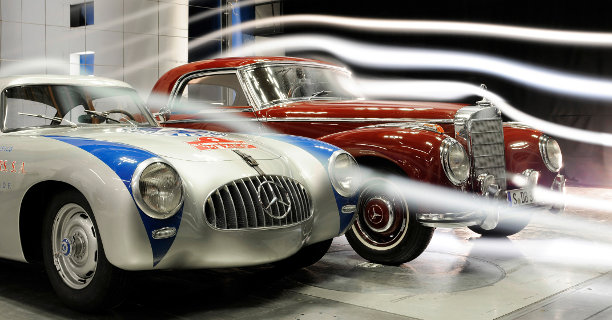
\includegraphics[width=0.618\textwidth]{pictures/aero}}
\title{Differentialgleichungen}
\subtitle{The Core of the Whole Business}
\author{}
\date{}
%\lowertitleback{
%\includegraphics[height=1.1cm]{/Users/jormawassmer/Pictures/logokoeniz.jpg}%
%\copyright Jorma Wassmer
%1. Auflage, Februar 2011
%}


\begin{document}
\maketitle
\tableofcontents
%\thispagestyle{empty}
\cleardoublepage
%\setcounter{page}{1}

\section{Beispiele}

\begin{wrapfigure}{r}{0.382\textwidth}
\vspace{-0pt}
  \begin{center}
    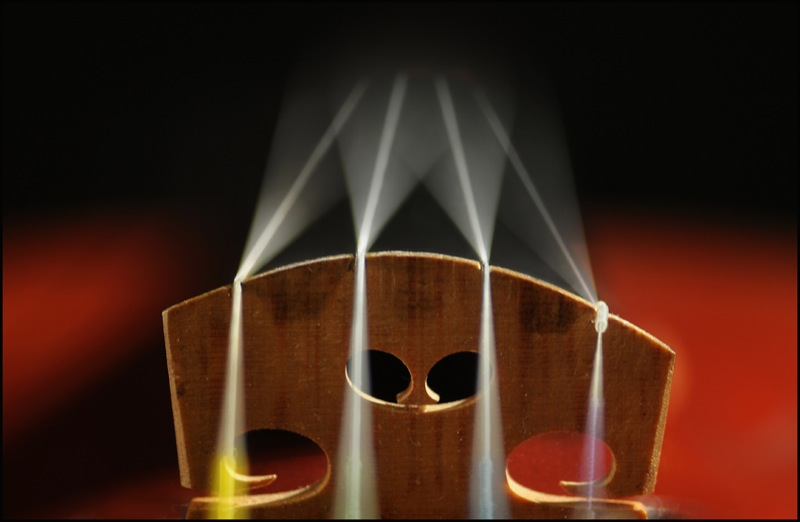
\includegraphics[width=0.37\textwidth]{pictures/geige}
  \end{center}
\caption{Geige}
\end{wrapfigure}
Wir besch\"aftigen uns hier mit --- wie der Name des Skripts sagt --- Differentialgleichungen, L\"osungsmethoden und Eigenschaften der L\"osungen. Wir verzichten vorerst auf eine formale Definition einer \glqq gew\"ohnlichen Differentialgleichung\grqq. Es handelt sich dabei um Gleichungen, in der eine Funktion $f$, Ableitungen von $f$ und eventuell noch Variablen, von denen $f$ abh\"angt, auftauchen.

\subsection{Problemstellung}

Als erstes, einfaches Beispiel betrachten wir die Gleichung
$$f'(x)=f(x).$$
Eine L\"osung kann leicht erraten werden.

\begin{ueb}
Nenne zwei m\"ogliche L\"osungen obiger Differentialgleichung.
\end{ueb}

Als Mathematiker ist man oft an der L\"osungsvielfalt interessiert. In andern Wissenschaften jedoch wird h\"aufig bloss eine L\"osung --- eine spezielle L\"osung, beispielsweise zu einem bekannten Anfangswert --- gesucht.

Bevor wir exemplarisch typische zus\"atzliche Anforderungen angeben und motivieren, m\"ochte ich durch eine schwammige Definition den  Begriff \glqq gew\"ohnliche Differentialgleichung\grqq\ abgrenzen.

\begin{defn}
Sucht man eine Funktion
$$f:\mR\longrightarrow\mR^n$$
und gibt eine Relation zwischen $f$ und den Ableitungen von $f$ an, so spricht man von einer \textbf{gew\"ohnlichen Differentialgleichung}.
\end{defn}


\begin{bem}
Betrachtet man hingegen Funktionen, die auf einem h\"oherdimensionalen Raum definiert sind
$$f:\mR^k\longrightarrow\mR^n$$
und gibt Beziehungen zwischen $f$ und den \emph{partiellen} Ableitungen von $f$ an, so handelt es sich um eine sogenannte partielle Differentialgleichung.
\end{bem}

Das Interesse an Differentialgleichungen ist schon alt, denn sie eignen sich hervorragend zum Modelllieren von Problemen der realen Welt; insbesondere physikalischer Natur. Diese Problemstellungen haben auch die Typen der oft untersuchten Gleichungen und der zus\"otzlichen Bedingungen, die man an die L\"osungen stellt um Eindeutigkeit zu erhalten, gepr\"agt. Jedoch k\"onnen die meisten Differentialgleichungen analytisch nicht in geschlossener Form gel\"ost werden. Analytische Methoden liefern aber oft Aufschluss \"uber qualitatives Verhalten wie Langzeitverhalten, Stabilit\"at etc. W\"ohrend das quantitative Verhalten heute recht bequem mit dem Computer untersucht werden kann, sind qualitative Aussagen fast ausschliesslich analytischen Untersuchungen zu verdanken. Fragestellungen von Anwendern verlangen oft beides. Deshalb wollen wir auch beide Vorgehensweisen ber\"uhren.

\subsection{Modellprobleme}

Bei einigen Problemen werde ich zur Begr\"undung, warum gerade die angegebene Differentialgleichung untersucht wird, physikalischen Hintergrund erl\"autern. Diese sind aber f\"ur das Verstehen der Mathematik nicht notwendig.

\subsubsection{Das mathematische Pendel}

Ein
\marginnote{
\qrcode{
https://www.youtube.com/watch?v=Yv2XERZNB-Y}
}
Pendel der L\"ange $L$ und Masse $m$ sei an einem festen Punkt $P$ aufgeh\"angt und schwinge in einer Ebene um die Ruhelage. Wir wollen den zeitlichen Verlauf dieser Bewegung studieren. Bei der zu beschreibenden Bewegung reicht es offensichtlich, die Winkelauslenkung $\varphi$ zu jedem Zeitpunkt $t$ anzugeben; wir suchen also $\varphi(t)$. Wie erh\"alt man eine Gleichung f\"ur $\varphi$?

\begin{figure}
\begin{center}
\definecolor{qqwuqq}{rgb}{0.13,0.13,0.13}
\definecolor{qqqqff}{rgb}{0.33,0.33,0.33}
\begin{tikzpicture}[line cap=round,line join=round,>=triangle 45,x=1.0cm,y=1.0cm]
\clip(-4.04,-2.96) rectangle (2.86,4.46);
\draw [shift={(0,4)},color=qqwuqq,fill=qqwuqq,fill opacity=0.1] (0,0) -- (-129.12:1) arc (-129.12:-90:1) -- cycle;
\draw [shift={(0,4)}] plot[domain=4.03:5.39,variable=\t]({1*3.87*cos(\t r)+0*3.87*sin(\t r)},{0*3.87*cos(\t r)+1*3.87*sin(\t r)});
\draw (0,4)-- (0,0.13);
\draw [->] (0,4) -- (-3.88,-0.8);
\draw [->] (-2.44,1) -- (-2.44,-1.96);
\draw [->] (-2.44,1) -- (-1.1,0);
\begin{scriptsize}
\fill [color=qqqqff] (-2.44,1) circle (3pt);
\draw[color=qqwuqq] (-2.8,1.1) node {$m$};
\draw[color=qqwuqq] (-1.65,2.4) node {$L$};
\draw[color=qqwuqq] (-0.25,3.3) node {$\varphi$};
\fill [color=qqqqff] (0,4) circle (1.5pt);
\draw[color=qqwuqq] (0.2,4.1) node {$P$};
\end{scriptsize}
\end{tikzpicture}
\end{center}
\caption{Das mathematische Fadenpendel}
\end{figure}

Offensichtlich wirkt auf $m$ die Kraft $F_G=mg$ mit $g$ als Ortsfaktor, wobei der radiale Anteil daf\"ur sorgt, dass die Schnur gespannt bleibt, und der Winkelanteil $mg\sin(\varphi)$ f\"ur die Winkelbeschleunigung $L\varphi''$ verantwortlich ist. Damit ergibt sich
$$mL\varphi''(t)=-mg\sin(\varphi(t)).$$
Mit dem negativen Vorzeichen weisen wir darauf hin, dass die Kraft r\"ucktreibend ist. Formen wir die Gleichung nach $\varphi''$ um und benutzen die bekannte N\"aherung f\"ur kleine Winkel, $\sin(\ga)\approx\ga$, so haben wir
\begin{equation}\label{eq:mathpendel}
\varphi''(t)=-\frac{g}{L}\varphi(t).
\end{equation}
Setzt man
$$\go_0=\sqrt{\frac{g}{L}}$$
ergibt sich als L\"osung
$$\varphi(t)=c_1\sin(\go_0 t)+c_2\cos(\go_0 t),$$
wobei $c_1,c_2\in\mR$ beliebig sind.
Man erkennt, dass f\"ur eine Anfangsauslenkung und eine Anfangsgeschwindigkeit eine eindeutige L\"osung vorliegt.

\begin{ueb}
Pr\"ufe obige L\"osung durch Einsetzen in \eqref{eq:mathpendel}.
\end{ueb}

\subsubsection{Der radioaktive Zerfall}

Durch
\marginnote{
\qrcode{
https://www.youtube.com/watch?v=x1g-JJ5gWuA}
}
Beobachtungen stellt man fest, dass die Anzahl Zerf\"alle proportional zur noch vorhandenen Stoffmenge $N$ ist. Bezeichnen wir mit $N(t)$ den zum Zeitpunkt $t$ noch verbleibenden Rest und mit $N_0$ die Stoffmenge zur Zeit $t=0$. Dann haben wir
\begin{equation}\label{eq:radiozerfall}
N'(t)=-kN(t)
\end{equation}
f\"ur ein $k\in\mR^+$. Das negative Vorzeichen in \eqref{eq:radiozerfall} interpretiert die Abnahme mit zunehmender Zeit. Wie im ersten Beispiel kann man eine L\"osung sofort hinschreiben:
$$N(t)=c\mathrm{e}^{-kt}.$$

\begin{ueb}
\"Uberlege kurz, dass mit unserer Notation $c=N_0$ gilt.
\end{ueb}

Wie lange dauert es, bis sich die Menge der radioaktiven Substanz halbiert hat? Bezeichnen wir mit $T$ diese Zeit, so erhalten wir
$$T=\frac{\ln(2)}{k}$$
und stellen freudig fest, dass $T$ unabh\"angig von $N_0$ ist. In der Euphorie geben wir $T$ den suggestiven Namen \emph{Halbwertszeit}. Sie charakterisiert f\"ur ein Element den Zerfallsprozess.

\begin{ueb}
Leite die Formel $T=\frac{\ln(2)}{k}$ her.
\end{ueb}

\begin{bem}
Allgemein f\"uhren Wachstums- und Zerfallsprozesse, bei denen die Ver\"anderung proportional zur gegenw\"artigen Gr\"osse ist, auf Differentialgleichungen zu \eqref{eq:radiozerfall} \"ahnlicher Gestalt.
\end{bem}

\subsubsection{Bev\"olkerungswachstum}

Das
\marginnote{
\qrcode{
https://www.youtube.com/watch?v=knQOOsgjbYg}
}
Wachstum einer Bev\"olkerung ist eine Frage von eminenter Bedeutung, sowohl in der Medizin, in der Zoologie, aber auch f\"ur die Menschheit.
Ein einfaches Modell zur Beschreibung einer Population $p$ ohne nat\"urliche Feinde ist, dass sowohl die Geburtenzahl, wie auch die Sterbezahl proportional zur Gr\"osse der Bev\"olkerung sind. Dann gibt es eine Geburtenrate $B$, eine Sterberate $D$ und $p$ gen\"ugt der Gleichung
\begin{equation}\label{eq:population}
p'=Bp-Dp.
\end{equation}
Mit $\gb=B-D$ in \eqref{eq:population} erh\"alt man via $k=-\gb$ einen Wachstumsprozess vom Typ \eqref{eq:radiozerfall} mit Verdoppelungszeit $T=\ln(2)/\gb$. Beobachtet man aber in der Realit\"at ein Wachstum, das noch st\"arker ist --- Verk\"urzung der Verdoppelungszeiten --- dann ist \eqref{eq:population} kein geeignetes Modell. Ein schwerer Nachteil dieses Modells ist die Vorhersage grenzenlosen Wachstums. Dies kann wegen der Endlichkeit aller Dinge nicht vorliegen. Nun erweitert man das Modell durch einen sogenannten Stressfaktor $S$, der proportional zur Anzahl Begegnungen von Individuen der Bev\"olkerung ist, welche selbst proportional zu $p^2$ ist. Damit hat man
\begin{equation}\label{eq:populationstress}
p'=\gb p-Sp^2.
\end{equation}
Mit $p(t)=\frac{\gb}{S}$
verf\"ugt man \"uber eine konstante L\"osung. Es ergibt sich sogar, dass jede L\"osung sich an diese konstante L\"osung ann\"ahert. Man erh\"alt dies, indem man zu jedem Anfangswert eine L\"osung durch diesen Anfangswert angibt, die diese Eigenschaft hat. Aus der Eindeutigkeit, die wir noch zeigen werden, folgt dann die Behauptung. Man bekommt die L\"osung f\"ur einen beliebigen Anfangswert mit der Methode der \emph{Trennung der Ver\"anderlichen}.

Nehmen wir an, es gibt eine L\"osung $p(t)$ mit $p_0\neq\gb/S$. Ist $\gb p-Sp^2\neq0$ liefert \eqref{eq:populationstress}
$$\frac{\mathrm{d}p}{\mathrm{d}t}\frac{1}{\gb p-Sp^2}=1.$$
Integration von $t_0$ bis $t$ liefert
$$\int_{t_0}^t\frac{\mathrm{d}p(s)}{\mathrm{d}t}\frac{\mathrm{d}s}{\gb p(s)-Sp(s)^2}=\int_{t_0}^t\,\mathrm{d}s=t-t_0.$$
Ist $\gb p-Sp^2\neq0$, so ist auch $p'\neq0$ und die linke Seite ergibt mit der Substitutionsregel
$$\int_{p_0}^p\frac{\mathrm{d}z}{\gb z-Sz^2}.$$
Dies wird mittels einer Partialbruchzerlegung integriert.
\begin{ueb}
Zeige, dass mit $K=\gb/S$
$$\frac{1}{\gb z-Sz^2}=\frac{1}{\gb}\cdot\left(\frac{1}{z}+\frac{1}{K-z}\right)$$
gilt.
\end{ueb}
\noindent Wir erhalten mit $K=\gb/S$
\begin{equation}\label{partint}
\begin{split}
\frac{1}{\gb}\int_{p_0}^p\frac{1}{z}+\frac{1}{K-z}\,\mathrm{d}z=\qq\qq\\
=\frac{1}{\gb}\left(\ln\left(\frac{\abs{p}}{\abs{p-K}}\right)-\ln\left(\frac{\abs{p_0}}{\abs{p_0-K}}\right)\right).
\end{split}
\end{equation}
\begin{ueb}
Zeige: Wegen $p_0,p>0$ erh\"olt man f\"ur den Ausdruck \eqref{partint} die Form
$$\frac{p(p_0-K)}{(p-K)p_0}=\mathrm{e}^{\gb(t-t_0)}.$$
\end{ueb}
\noindent Daraus folgt
\begin{equation}\label{eq:bruch}
p(1-B)=-BK.
\end{equation}
Schliesslich erhalten wir die L\"osung
$$p(t)=\frac{Kp_0}{p_0-\mathrm{e}^{-\gb(t-t_0)}(p_0-K)}.$$

\begin{ueb}
Leite die L\"osung her, indem du \eqref{eq:bruch} nach $p$ aufl\"ost, den Bruch ausschreibst und danach mit $\mathrm{e}^{-\gb(t-t_0)}$ erweiterst.
\end{ueb}

\begin{ueb}
Untersuche die Qualit\"at der L\"osung. Erf\"ullt $p(t_0)$ die Erwartungen. Wie siehts in ferner Zukunft aus, d.h. $t\to\infty$? Wie sahs in der Vergangenheit aus (betrachte die F\"alle $p_0\in(0,K)$ und $p_0>K$)?
\end{ueb}

\begin{bem}
Die hier behandelte Gleichung wird oft \textbf{logistische Gleichung} genannt.
\end{bem}

\subsubsection{Die schwingende Saite}

\begin{bem}
An diesem Beispiel m\"ochte ich zeigen, dass gew\"ohnliche Differentialgleichungen eine erhebliche Rolle bei der Diskussion von Eigenschaften von L\"osungen partieller Differentialgleichungen spielen.
\end{bem}

Bei einer schwingenden Saite sucht man eine Funktion $u$, die die Auslenkung zum Zeitpunkt $t$ an der Stelle $x$ beschreibt; also
$$u(t,x).$$
Ohne Begr\"undung gebe ich die zugrundeliegende partielle Differentialgleichung an. Sie lautet
\begin{equation}\label{eq:saite}
\frac{\partial^2u}{\partial t^2}=\lambda^2\frac{\partial^2u}{\partial x^2}.
\end{equation}
Die Saite sei an den Endpunkten $x=0$ bzw. $x=\pi$ befestigt. Damit erh\"olt man die Randbedingungen $u(t,0)=u(t,\pi)=0$. Der Einfachheit halber setzen wir $\lambda=1$.
Mit dem Ansatz
$$u(t,x)=v(x)\cdot w(t)$$
erh\"alt man die Beziehung
$$v(x)w''(t)=v''(x)w(t).$$
Betrachten wir einen Punkt $(t,x)$, in dem beide Funktionen nicht verschwinden, so k\"onnen wir
$$\frac{w''(t)}{w(t)}=\frac{v''(x)}{v(x)}$$
schreiben. Da die beiden Seiten von verschiedenen Variablen abh\"angen, m\"ussen sie konstant und gleich sein. Also in der Art
\begin{align*}
w''&=-Kw\\
v''&=-Kv
\end{align*}
mit $K>0$. Das Vorzeichen ist wiederum physikalisch motiviert. Sonst erh\"alt man keine zeitlich periodische L\"osung. F\"ur eine vollst\"andige L\"osung m\"usste man aus mathematischer Sicht auch den andern Fall diskutieren. Wie in \eqref{eq:mathpendel} lautet eine L\"osung der zweiten Gleichung
$$v(x)=c_1\cos(\sqrt{K}x)+c_2\sin(\sqrt{K}x).$$

\begin{ueb}
\"Uberlege dir, dass mit den Randbedingungen der Cosinusterm verschwindet und $K=n^2$ mit $n\in\mN$ gelten muss, so dass also
$$v(x)=c_2\sin(nx)$$
wird.
\end{ueb}

\noindent Damit kann man eine Schar von L\"osungen der Gleichung \eqref{eq:saite} angeben, n\"amlich
$$u(t,x)=\sum_{n=0}^\infty\left(d_n^1\cos(nt)+d_n^2\sin(nt)\right)\sin(nx).$$

\begin{ueb}
Geht man von einer Ausgangslenkung mit Anfangsgeschwindigkeit $0$ aus, so erh\"alt man
$$u(t,x)=\sum_{n=0}^\infty d_n\cos(nt)\sin(nx).$$
\end{ueb}

Auf Seite \pageref{fig:saite} findet man eine mögliche Lösung in Abbildung \ref{fig:saite} geplottet.

\subsubsection{Die W\"armeleitungsgleichung}

Wir betrachten die eindimensionale W\"arme\-lei\-tungs\-gleichung, die die Temperaturentwicklung in einem Stab modelliert. Wir nehmen an, wir h\"atten einen Stab der L\"ange $l$. F\"ur $x\in(0,l)$ und $t\in\mR$ sei $u(x,t)$ die Temperatur des Stabes zum Zeitpunkt $t$ an der Stelle $x$. Die Anfangsverteilung der Temperatur sei durch eine Funktion $u_0(x)$ gegeben. An den Enden des Stabes bieten sich verschiedene Randbedingungen an, die physikalisch motiviert sind. Zum einen kann man annehmen, dass man an den Enden eine feste Temperatur $T$ hat, o.E.d.A. nehmen wir $T=0$
an, oder eine vollst\"andige Isolierung, d.h. keine Temperatur\"anderung durch den Rand: $u_x(0,t)=u_x(l,t)=0$ f\"ur alle $t\in\mR$. An der
Stelle $(x,t)$ ist dabei die Differentialgleichung
$$\frac{\partial u}{\partial t}=k\frac{\partial^2 u}{\partial^2 x}$$
erf\"ullt. Wiederum setzen wir $k=1$ und brauchen den Ansatz $u(x,t)=v(x)w(t)$. Man erh\"alt
$$\frac{w'}{w}=\frac{v''}{v}=\lambda.$$
Hier lautet eine m\"ogliche L\"osung
$$u(x,t)=\mathrm{e}^{\lambda t}(c_1\cos(\sqrt{\lambda}x)+c_2\sin(\sqrt{\lambda}x)).$$
Aus der Randbedingung links ergibt sich $c_1=0$, und die Bedingung rechts liefert $\sin(\sqrt{\lambda}l)=0$, also
$$\lambda=\frac{n^2\pi^2}{l^2}$$
f\"ur ein $n\in\mN$. Da man beliebige Summen bzw. Reihen bilden kann, lautet eine allgemeinere L\"osung
$$u(x,t)=\sum_{n=0}^\infty c_n\mathrm{e}^{\frac{n^2\pi^2}{l^2}t}\sin\left(\frac{n\pi}{l}x\right).$$
Die Werte f\"ur $c_n$ bestimmt man durch Entwicklung von $u_0$ in eine Fourierreihe.
\marginnote{
\qrcode{
https://www.youtube.com/watch?v=QY7fD_fFYnk}
}

\subsubsection{Das elektrische Feld}

Sei $\V{E}$ ein elektrisches Feld in der Ebene.
\marginnote{
\qrcode{
https://youtu.be/0zcRz1kphBQ}
}
Sei $\V{U}$ das Potential dieses Feldes. Also $\V{E}=\nabla\V{U}$, wobei $\V{U}$ eine Funktion der beiden unabh\"angigen Ver\"anderlichen $x,y$ ist. Welches sind die Linien, l\"angs denen das Potential konstant ist? In fast allen Punkten $(x,y)$ wird entweder $x = x(y)$ eine Funktion von $y$ sein, oder umgekehrt $y = y(x)$ eine Funktion von $x$.
Wir beschr\"anken uns auf den zweiten Fall, der erste geht daraus durch einfaches Umschreiben hervor.
Um die \"Aquipotentiallinien zu finden, geben wir uns eine, zun\"achst beliebige, Konstante $c$ vor und stellen die Frage, wo ist $\V{U}= c$? Die Annahme, dass diese Linie durch $y = y(x)$ zu beschreiben ist, f\"uhrt auf
$$\frac{\partial\V{U}}{\partial x}+\frac{\partial\V{U}}{\partial y}\frac{\mathrm{d}y}{\mathrm{d}x}=0.$$
Dies ist ein Beispiel einer sogenannten exakten Differentialgleichung.

\begin{ueb}
\"Uberlege kurz, dass obige Gleichung Sinn macht.
\end{ueb}

\begin{defn}
Die
\marginnote{
\qrcode{
https://www.youtube.com/watch?v=haiyzr8B7_A}
}
Differentialgleichung der Form
\begin{equation}\label{eq:exakt}
f(x,y)\frac{\mathrm{d}y}{\mathrm{d}x}+g(x,y)=0
\end{equation}
heisst \textbf{exakt}, wenn es eine Funktion $U:\mR^2\longrightarrow\mR$ gibt, so dass
\begin{equation}\label{eq:exaktbed}
f(x,y)=\frac{\partial U}{\partial y}\q\text{und}\q g(x,y)=\frac{\partial U}{\partial x}.
\end{equation}
\end{defn}
\noindent Aus $U_{xy}=U_{yx}$ erh\"alt man unmittelbar die notwendige Bedingung $f_x=g_y$ f\"ur die Exaktheit der Gleichung. Ist bei einer Gleichung der Form \eqref{eq:exakt} die Bedingung \eqref{eq:exaktbed} nicht erf\"ullt, so ist es manchmal m\"oglich, einen \textbf{integrierenden Faktor} zu finden. Dies ist eine Funktion $M(x,y)$, so dass $Mf$ bzw. $Mg$ die Bedingung \eqref{eq:exaktbed} erf\"ullen. Eine Diskussion der Gleichung ist dann der Diskussion einer exakten Gleichung \"ahnlich. Insbesondere f\"uhrt die Forderung $(Mg)_y=(Mg)_x$ auf die partielle Differentialgleichung
$$M_yg+Mg_y=M_xf+Mf_x.$$

\newpage

\section{L\"osungsmethoden}
\subsection{Lineare Differentialgleichungen}

\begin{defn}
Eine Differentialgleichung der Form
%\begin{multline*}
$$a_n(x)y^{(n)}(x)+a_{n-1}(x)y^{(n-1)}(x)+%\dots\\
\dots+a_0(x)y(x)=b(x)$$
%\end{multline*}
heisst \textbf{lineare Differentialgleichung $n$-ter Ordnung}, wobei $a_n(x),\dots,a_0(x)$ und $b(x)$ Funktionen sind.
\end{defn}
\begin{bsp}
Ein Spezialfall einer linearen Differentialgleichung zweiter Ordnung mit konstanten Koeffizienten ist
$$a_2y''(x)+a_1y'(x)+a_0y(x)=b(x).$$
Der von $x$ abh\"angige Ausdruck $b(x)$ wird \textbf{St\"orterm} genannt.
\end{bsp}
\begin{defn}
Ist $b(x)=0$, so heisst die Differentialgleichung \textbf{homogen}, andernfalls wird sie \textbf{inhomogen} genannt.
\end{defn}
\begin{bem}
F\"ur einige explizite Differentialgleichungen erster Ordnung gibt es Standardverfahren zu ihrer numerischen L\"osung. Viele explizite Differentialgleichungen h\"oherer Ordnung lassen sich in ein System von Differentialgleichungen erster Ordnung \"uberf\"uhren, auf die dann diese Standardverfahren angewendet werden d\"urfen.
\end{bem}
\begin{bsp}
Sei
$$y^{(n)}+a_{n-1}y^{(n-1)}+\dots+a_1y'+a_0y=b(x)$$
eine DGL $n$-ter Ordnung. Diese l\"asst sich in ein DGL-System verwandeln. Wir setzen
\begin{align*}
y_1&=y, y_2=y',\dots,y_n=y^{(n-1)}\\
b_1&=\dots=b_{n-1}=0, b_n=b(x)
\end{align*}
F\"ur $n=4$ erhalten wir zum Beispiel
\begin{align*}
y_1'&=\phantom{-a_0y_1-a_1}y_2\\
y_2'&=\phantom{-a_0y_1-a_1y_2-a_2}y_3\\
y_3'&=\phantom{-a_0y_1-a_1y_2-a_2y_3-a_3}y_4\\
y_4'&=-a_0y_1-a_1y_2-a_2y_3-a_3y_4+b(x)
\end{align*}
\end{bsp}

\subsection{Lineare Differentialgleichungssysteme}

\begin{bsp}
Gegeben sei das Differentialgleichungssystem
\marginnote{
\qrcode{
https://www.youtube.com/watch?v=Tbhw2Se259U}
}
\begin{align*}
y_1'&=7y_1-5y_2\\
y_2'&=4y_1-2y_2
\end{align*}
das heisst
$$\vec{y}\,'=
\begin{pmatrix}
7 & -5\\
4 & -2
\end{pmatrix}
\vec{y}.$$
Staunen Sie nun, wie man die L\"osungen bestimmen kann:
Wir finden die Eigenwerte via
$$(\gl-7)(\gl+2)+20=0.$$
Das ergibt $\gl_1=2, \gl_2=3$. Daraus erh\"alt man die Eigenvektoren
$$\vec{v_1}=\pv{1}{1}\q\text{und}\q\vec{v_2}=\pv{5}{4}.$$

Dies liefert das Fundamentalsystem der L\"osungen
$$\vec{y_1}=\mathrm{e}^{2x}\pv{1}{1},\q\vec{y_2}=\mathrm{e}^{3x}\pv{5}{4}.$$
\end{bsp}

\begin{ueb}
Rechne Eigenwerte und Eigenvektoren nach.
\end{ueb}


\begin{ueb}
Zeige, dass $c_1\vec{y_1}+c_2\vec{y_2}$ das Gleichungssystem erfüllt.
\end{ueb}

\subsection{Die Traktrix}

\begin{wrapfigure}{r}{0.4\textwidth}
\vspace{-5pt}
\begin{center}
\definecolor{xdxdff}{rgb}{0.3,0.3,0.3}
\scalebox{0.9}{
\begin{tikzpicture}[line cap=round,line join=round,>=triangle 45,x=1.0cm,y=1.0cm]
\draw[->,color=black] (-1.9,0) -- (4.94,0);
\foreach \x in {-1,1,2,3,4}
\draw[shift={(\x,0)},color=black] (0pt,-2pt);
\draw[color=black] (4.6,0.08) node [anchor=south west] { x};
\draw[->,color=black] (0,-1.94) -- (0,6.3);
\foreach \y in {-1,1,2,3,4,5,6}
\draw[shift={(0,\y)},color=black] (2pt,0pt) -- (-2pt,0pt);
\draw[color=black] (-0.1,5.9) node [anchor=east] { y};
\clip(-1.9,-1.94) rectangle (4.94,6.3);
\draw[smooth,samples=100,domain=0.02:2.9] plot(\x,{3*ln((3+(9-(\x)^2)^0.5)/(\x))-(9-(\x)^2)^0.5});
\draw (0,4)-- (1.5,1.35);
\draw [dotted] (0,1.35)-- (1.5,1.35);
\draw [dotted] (1.5,1.35)-- (1.5,0);
\begin{scriptsize}
\fill [color=xdxdff] (0,4) circle (1.5pt);
\draw[color=xdxdff] (0.14,4.26) node {$Z$};
\fill [color=xdxdff] (1.5,1.35) circle (1.5pt);
\draw[color=xdxdff] (1.64,1.62) node {$P$};
\end{scriptsize}
\end{tikzpicture}
}
\end{center}
\caption{Die Traktrix}
\vspace{-5pt}
\end{wrapfigure}
In
\marginnote{
\qrcode{
https://www.youtube.com/watch?v=7c4ajQ6n39w}
}
der $xy$-Ebene ziehe man einen Punkt $P\point{x}{y}$ an einer Schnur $PZ$ der L\"ange $a$. $Z$ soll auf der positiven $y$-Achse fortr\"ucken, und zu Beginn befinde sich $P$ in $(a,0)$. Welche Kurve beschreibt $P$?
Wir suchen eine Funktion $y=y(x)$ mit $\abs{Z-P}=a$. Betrachtet man den Steigungswinkel erh\"alt man f\"ur den Punkt $P$
$$y'=-\frac{Z-y}{x}.$$
Ferner gilt
$$Z-y=\sqrt{a^2-x^2}$$ und damit
$$y'=-\frac{\sqrt{a^2-x^2}}{x}.$$
Mit der Bedingung $y(a)=0$ erh\"alt man als L\"osung
$$y(x)=a\cdot\ln\left(\frac{a+\sqrt{a^2-x^2}}{x}\right)-\sqrt{a^2-x^2}.$$

\begin{ueb}
\"Uberpr\"ufe die L\"osung.
\end{ueb}

\subsection{Isoklinenverfahren}

\"Uber die Differentialgleichung
$$y'=f(x,y)$$
ist jedem Punkt der $xy$-Ebene eine Richtung $y'=\tan(\ga)$ zugeordnet. W\"ahlt man f\"ur $y'$ einen festen Wert,
$$y'=c=f(x,y),$$
so beschreibt diese Gleichung eine Kurve in der Ebene.
Diese Kurven heissen \textbf{Isoklinen}, also Kurven gleicher Neigung. Durch Zeichnung von gen\"ugend vielen Richtungsstrecken erh\"alt man ein Richtungsfeld, in das man n\"aherungsweise L\"osungskurven der Differentialgleichung eintragen kann.

\begin{ueb}
Zeichne f\"ur
$$y'=-\frac{y}{x}$$
einige Isoklinen und damit m\"ogliche L\"osungskurven.
\end{ueb}

\subsection{Trennung der Variablen}

Viele Differentialgleichungen erster Ordnung lassen sich auf die Form
$$y'=f(x)\cdot g(y)$$
bringen.
F\"ur diesen Typ l\"osst sich das Problem auf ein Integrationsproblem zur\"uckf\"uhren, das aber nicht unbedingt eine analytische L\"osung haben muss.
\marginnote{
\qrcode{
https://www.youtube.com/watch?v=x1g-JJ5gWuA}
}
Man schreibt $y'$ als Quotient der Differentiale $\mathrm{d}y/\mathrm{d}x$
$$\frac{\mathrm{d}y}{\mathrm{d}x}=f(x)\cdot g(y)$$
und trennt dann die Variablen:
$$\frac{1}{g(y)}\,\mathrm{d}y=f(x)\,\mathrm{d}x.$$
Durch Integration beider Seiten erh\"alt man die L\"osungen der Differentialgleichung, n\"amlich
$$\int\frac{1}{g(y)}\,\mathrm{d}y=\int f(x)\,\mathrm{d}x.$$
Auch wenn die Integrale keine elementare L\"osung haben gilt die Differentialgleichung als gel\"ost.

\begin{ueb}
L\"ose
$$y'=(x^2+1)(y-2).$$
\end{ueb}

\begin{ueb}
L\"ose mit der Methode der Trennung der Variablen
\begin{enumeratea}
\item $u'=u^2+1$
\item $u'=-\frac{x^2}{u^3}$
\item $u'=\mathrm{e}^u\sin(x)$
\end{enumeratea}
und diskutiere das Verhalten der L\"osungen mit $u(0)=p_0$ wobei $p_0\in\mR$. Darunter verstehen wir die Beantwortung folgender Fragen.
\begin{itemize}
\item F\"ur welche $t\in\mR$ existiert eine L\"osung?
\item Wie verh\"alt sich die L\"osung f\"ur $t\to t_+$ bzw. $t\to t_-$, wenn $(t_-,t_+)$ das Intervall bezeichnet, auf dem die L\"osung $u(t)$ existiert?
\end{itemize}
\end{ueb}

\subsection{Substitution}

Hat die Funktion $f(x,y)$ noch nicht die f\"ur eine Trennung der Variablen erforderliche Form eines Produkts, so l\"asst sich diese Form h\"aufig durch eine Substitution erreichen. Wir betrachten hier den Spezialfall, dass die Variablen $x,y$ immer in der folgenden Form auftreten:
$$\frac{ax+by+c}{dx+ey+f}=z.$$
Wir setzen $y'=f(x,y)=g(z)$ und unterscheiden f\"ur den Nachweis, dass dann immer eine Trennung der Variablen m\"oglich ist, zwei F\"alle. Sei $D=ae-bd$ die Determinante von
$$\begin{pmatrix}
a & b\\
d & e
\end{pmatrix}.$$

\subsubsection{D gleich 0}

Falls $b=0=e$, so h\"angt $g(z)$ nur noch von $x$ ab und die Variablen sind getrennt. Sei daher $b\neq0$ oder $e\neq0$.

\begin{description}
\item[Fall a)] Sei $b\neq0$. Dann setzen wir
$$u=ax+by+c.$$
Aus $D=0$ folgt, dass es eine Zahl $k$ gibt, so dass $d=ka$ \emph{und} $e=kb$. Daraus folgt
\begin{align*}
z &= \frac{ax+by+c}{dx+ey+f}\\
 &= \frac{ax+by+c}{k(ax+by+c)-kc+f}\\
 &= \frac{u}{ku+f-kc}
 \end{align*}
 Nun hat man f\"ur die Ableitung von $u$
\begin{align*}
\frac{\mathrm{d}u}{\mathrm{d}x}&=a+b\frac{\mathrm{d}y}{\mathrm{d}x}=a+bg(z)\\
&=a+bg\left(\frac{u}{ku+f-kc}\right)
\end{align*}
 Die rechte Seite h\"angt nur noch von $u$ ab, d.h. eine Trennung der Variablen ist erreicht.
 \item[Fall b)] Sei $b=0$ und $e\neq0$. Dann substituiert man den Nenner mit
 $$u=dx+ey+f.$$
 Aus $D=0$ und $b=0$ folgt $a=0$. Also
 $$z=\frac{c}{dx+ey+f}=\frac{c}{u}$$
 und f\"ur die Ableitung
\begin{align*}
\frac{\mathrm{d}u}{\mathrm{d}x}&=d+e\frac{\mathrm{d}y}{\mathrm{d}x}=d+eg(z)\\
&=d+eg\left(\frac{c}{u}\right)
\end{align*}
Damit sind wir fertig.
 \end{description}
 
 \subsubsection{D ungleich 0}
 
 Wir setzen
 $$ax+by+c=0\q\text{und}\q dx+ey+f=0$$
 Wegen $D\neq0$ ergibt das eine eindeutige L\"osung $(x_0,y_0)$. Wir setzen $x=x_0+v$ und $y=y_0+w$.
 \begin{align*}
z &= \frac{ax+by+c}{dx+ey+f}\\
&=\frac{ax_0+by_0+c+av+bw}{dx_0+ey_0+f+dv+ew}\\
&=\frac{av+bw}{dv+ew}
\end{align*}
Anschliessend setzt man $u=\frac{w}{v}$ woraus
$$z=\frac{a+bu}{d+eu}$$
folgt. Nun leiten wir ab
\begin{align*}
\frac{\mathrm{d}u}{\mathrm{d}x}&=\frac{v\frac{\mathrm{d}w}{\mathrm{d}x}-w\frac{\mathrm{d}v}{\mathrm{d}x}}{v^2}\\
&=\frac{v\frac{\mathrm{d}y}{\mathrm{d}x}-w}{v^2}\\
&=\frac{1}{v}\frac{\mathrm{d}y}{\mathrm{d}x}-\frac{u}{v}=\frac{1}{v}(g(z)-u)
\end{align*}
Das heisst
$$\frac{\mathrm{d}u}{g(z(u))-u}=\frac{\mathrm{d}v}{v}$$
und wir haben wiederum die Variablen getrennt.

\begin{ueb}
L\"ose
$$y'=\frac{x-2y+1}{2x-4y-1}$$
und \"uberzeuge dich davon, dass die L\"osung eine Parabel ist.
\end{ueb}

\begin{ueb}
L\"ose
$$y'=\frac{x+y}{x-y}$$
und schreibe die L\"osung in der Form $\frac{y}{x}$. Wechsle anschliessend zu Polarkoordinaten und notiere $\varphi(r)$. \"Uberzeuge dich davon, dass das Resultat eine Spirale ist.
\end{ueb}

\subsection{Variation der Konstanten}

Die linear Differentialgleichung
$$y'+g(x)y=s(x)$$
wobei $s(x)$ eine sogenannte St\"orfunktion ist, wird in zwei Schritten gel\"ost.

\begin{enumerate}
\item Man l\"ost die zugeordnete homogene Differentialgleichung
$$y'+g(x)y=0$$
durch Trennung der Variablen.
\begin{align*}
\int\frac{dy}{y} &= -\int g(x)dx\\
\ln\abs{y} &= -\int g(x)dx\\
y &= ce^{-\int g(x)dx}
\end{align*}
mit $c\in\mR$.
\item Die
\marginnote{
\qrcode{
https://www.youtube.com/watch?v=uSb8s91nv_s}
}
Integrationskonstante $c$ wird als Funktion von $x$ angesetzt --- Variation der Konstanten.
$$y=c(x)e^{-\int g(x)dx}.$$
F\"ur die Ableitung erhalten wir
$$y' = c'(x)e^{-\int g(x)dx}+c(x)(-g(x))e^{-\int g(x)dx}$$
was
$$s(x)-g(x)y$$
entsprechen soll. Daraus folgt
$$c'(x)=s(x)e^{\int g(x)dx}$$
also
$$c(x)=\int s(x)e^{\int g(x)dx}dx+K$$
Die L\"osung lautet
$$y=e^{-\int g(x)dx}\cdot\left(\int s(x)e^{\int g(x)dx}dx+K\right).$$
\end{enumerate}

\begin{ueb}
L\"ose
$$y'-y\tan(x)=-\sin(x).$$
\end{ueb}

\begin{ueb}
L\"ose
$$y'+\frac{y}{x}=x^2+4$$
\end{ueb}

\subsubsection{Variation der Konstanten --- abstrakter}

Wir beschr\"onken uns auf den Fall eines einzigen Freiheitsgrades, den einzigen mit expliziten L\"osungsmethoden.

Sei $I\subset\mR$ ein offenes Intervall und $a,s:I\longrightarrow\mR$ stetige Funktionen. Wir studieren die Differentialgleichungen
\begin{align}
y' &= ay\\
y' &=ay+s
\end{align}

\begin{satz}
Die homogene lineare Differentialgleichung besitzt als L\"osung genau die Funktionen $y:I\longrightarrow\mR$ gegeben durch
$$y(x)=ce^{\int_{x_0}^xa(t)dt}$$
mit $c\in\mR$ und $x_0\in I$.
\end{satz}

\begin{proof}
Dass die oben beschriebenen Funktionen $y$ die Gleichung erf\"ullen, erkennen wir durch Ableiten. F\"ur die Eindeutigkeit brauchen wir auch ein direktes Argument. Sei $y$ wie oben und $z$ eine weitere L\"osung, so ergibt sich
$$\frac{d}{dx}\frac{z}{y}=\frac{z'y-zy'}{y^2}=\frac{azy-zay}{y^2}=0.$$
Also ist $\frac{z}{y}$ konstant und somit $z=cy$.
\end{proof}

\begin{satz}
Die L\"osungen der inhomogenen linearen Differentialgleichung sind ein Nebenraum $N=L+d$ der L\"osungen der homogenen linearen Differentialgleichung $L$, wobei $d$ eine partikul\"ore L\"osung der inhomogenen Gleichung ist.
\end{satz}

\begin{proof}
Um $d$ zu erhalten bedienen wir uns der Formel
$$d(x)=c(x)e^{\int_{x_0}^xa(t)dt}$$
mit
$$c(x)=\int_{x_0}^xs(t)e^{-\int_{t_0}^ta(\gt)d\gt}dt,$$
wobei $x_0,t_0\in I$ beliebig gew\"ohlt werden d\"urfen.
Sie kann aus einer L\"osung $L$ durch Variation der Konstanten gewonnen werden. Wir hatten
$$y(x)=c(x)e^{\int_{x_0}^xa(t)dt}$$
und es soll die inhomogene lineare Differentialgleichung erf\"ullt sein. Also
\begin{align*}
y'(x) &=c'(x)e^{\int_{x_0}^xa(t)dt}+c(x)a(x)e^{\int_{x_0}^xa(t)dt}\\
&=a(x)y(x)+s(x).
\end{align*}
Dies liefert die Bedingung
$$c'(x)e^{\int_{x_0}^xa(t)dt}=s(x)$$
woraus sich $c'(x)$ und damit die Behauptung ergibt.
\end{proof}

\begin{kor}
F\"ur $t_0\in I$ und $x_0\in\mR$ existiert genau eine L\"osung $c$ der inhomogenen linearen Differentialgleichung mit $c(t_0)=x_0$.
\end{kor}

\begin{proof}
Dies ergibt sich unmittelbar aus den oben stehenden Betrachtungen.
\end{proof}

\subsection{Exakte Gleichungen}

Hier folgt noch einmal die Definition einer exakten Differentialgleichung.
\begin{defn}
Sei
\marginnote{
\qrcode{
https://www.youtube.com/watch?v=haiyzr8B7_A}
}
$\mG\subset\mR^n$ ein Gebiet. Die Differentialgleichung
$$Pdx+Qdy=0$$
mit $P,Q:G\longrightarrow\mR$ heisst \textbf{exakt}, wenn es eine stetig differenzierbare Funktion $F:G\longrightarrow\mR$ gibt, so dass $P=\frac{\partial F}{\partial x}=F_x$ und $Q=\frac{\partial F}{\partial y}=F_y$ gilt.
\end{defn}
\noindent Wir erhalten die L\"osungen, indem wir die Niveaulinien $F^{-1}(c)$ mit $c\in\mR$ nach der ersten oder zweiten Variablen aufl\"osen.

\begin{bem}
Eine L\"osung $F$ der obigen DGL heisst Potentialfunktion des Vektorfeldes $\point{P}{Q}$.
\end{bem}

Jetzt zu den in der Einleitung bereits erw\"ohnten integrierenden Faktoren. Wir setzen wiederum voraus, dass $G\subset\mR^2$ ein Gebiet ist, und $P:G\longrightarrow\mR$, $P:G\longrightarrow\mR$ Funktionen sind. Wenn nun die durch $(P,Q)$ definierte Differentialgleichung
\begin{equation}\label{eq:exakt2}
Pdx+Qdy=0
\end{equation}
nicht exakt ist, kann man versuchen, eine Funktion $M:G\longrightarrow\mR$ so zu bestimmen, dass
$$(MP)dx+(MQ)dy=0$$
exakt ist. Eine solche Funktion nennen wir einen \textbf{integrierenden Faktor} f\"ur \eqref{eq:exakt2}. Wenn man die Integrabilit\"otsbedingung $P_y=Q_x$ anwendet, erh\"olt man
$$\frac{\partial(MP)}{\partial y}=\frac{\partial(MQ)}{\partial x}$$
oder
$$M_yP+MP_y=M_xQ+MQ_x,$$
also eine partielle Differentialgleichung f\"ur $M$. Dies f\"uhrt zu Fragen, die ich hier nicht weiter untersuchen m\"ochte.

\begin{ueb}
Pr\"ufe, ob die Differentialgleichung
$$(\cos y+2xy)dx+(x^2-y-x\sin y)dy=0$$
exakt ist und l\"ose, wenn m\"oglich, in expliziter Form. Falls du nicht nach $y$ aufl\"osen kannst, l\"ose nach $x$.
\end{ueb}

\marginnote{
\qrcode{
https://www.youtube.com/watch?v=vaO64RJqjAk}
}

\begin{ueb}
Man \"uberpr\"ufe die folgenden Gleichungen auf Exaktheit. Falls nicht Exaktheit vorliegt, versuche einen integrierenden Faktor zu finden und bestimme die L\"osungen.
\begin{enumeratea}
\item $yy'=x$
\item $xy'=-y$
\item $x-y+(1-x)y'=0$
\item $4x+3y^2+2xyy'=0$
\item $xy^2+y-xy'=0$
\end{enumeratea}
\end{ueb}

Im Anhang findet ihr Abbildungen der Lösungen; ab Abbildung \ref{fig:potxxyy} auf Seite \pageref{fig:potxxyy}.

\subsection{Potenzreihenansatz}

Ohne ins Detail zu gehen akzeptieren wir folgenden
\begin{satz}
Wenn
\marginnote{
\qrcode{
https://www.youtube.com/watch?v=vkUnoLXzdvc}
}
die Koeffizienten einer Differentialgleichung Potenzreihen sind, dann auch die L\"osungen. Die L\"osungen haben zudem den gleichen Definitionsbereich wie die Koeffizientenfunktionen.
\end{satz}

\subsubsection{Die Hermite'sche Differentialgleichung}

Betrachte
\begin{equation}\label{eq:hermit}
y''-2xy'+\gl y=0
\end{equation}
mit $\gl\in\mR$. Mit dem Potenzreihenansatz
$$y(x)=\sum_{k=0}^\infty c_k\cdot x^k$$
erhalten wir die Bedingung
$$
(2c_2+\lambda c_0)
+\sum_{k=1}^\infty[(k+1)(k+2)c_{k+2}-2kc_k+\gl c_k]\cdot x^k=0,
$$
die wir wie folgt erf\"ullen k\"onnen. $c_0$ und $c_1$ k\"onnen frei gew\"ohlt werden, und f\"ur $k\geq0$ muss
$$c_{k+2}=\frac{2k-\gl}{(k+1)(k+2)}\cdot c_k$$
gelten. So erhalten wir
$$y(x)=c_0g(x)+c_1h(x)$$
mit
$$
g(x)=1-\frac{\gl}{2!}x^2
-\sum_{k=2}^\infty\frac{[4(k-1)-\gl][4(k-2)-\gl]\dotsm[4-\gl]\gl}{(2k)!}\cdot x^{2k}
$$
und
$$
h(x)=x
+\sum_{k=1}^\infty\frac{[4k-2-\gl][4(k-1)-2-\gl]\dotsm[2-\gl]}{(2k+1)!}\cdot x^{2k+1}.
$$
Besonders interessant ist der Fall $\gl=2n$ f\"ur $n\in\mN_0$. Wenn $n$ gerade ist, ist in diesem Fall $g=g_n$ ein gerades Polynom vom Grad $n$; wenn $n$ ungerade ist, ist $h=h_n$ ein ungerades Polynom vom Grad $n$. Man definiert die \emph{Hermite'schen Polynome} $H_n$ durch
$$H_n=(-1)^{n/2}\cdot2^{n/2}\cdot3\cdot5\dotsm(n-1)\cdot g_n,$$
f\"ur gerade $n$ und
$$H_n=(-1)^{(n-1)/2}\cdot2^{(n+1)/2}\cdot3\cdot5\dotsm n\cdot h_n,$$
falls $n$ ungerade ist.

\begin{ueb}
Kannst du die ersten paar Hermite'schen Polynome, vielleicht $H_0$ bis $H_3$, bestimmen?
\end{ueb}

\begin{bem}
Es wird gesagt, die Differentialgleichung \eqref{eq:hermit} trete in der Quantentheorie, beim Studium der Schwingungen von Molek\"ulen, auf.
\end{bem}

\begin{ueb}
Welche der folgenden Funktionen erf\"ullen die Hermite'sche Differentialgleichung?

\begin{minipage}{0.3\textwidth}
\begin{enumeratea}
\item $y=1$
\item $y=2x$
\end{enumeratea}
\end{minipage}
\begin{minipage}{0.4\textwidth}
\begin{enumeratea}
\setcounter{enumi}{2}
\item $y=-2+4x^2$
\item $y=-12x+8x^3$
\end{enumeratea}
\end{minipage}
\end{ueb}

\subsubsection{Die Legendre'sche Differentialgleichung}

Sie hat ihren Ursprung in der Astronomie und lautet
\begin{equation}\label{eq:legendre}
(1-x^2)y''-2xy'+\gl(\gl+1)y=0.
\end{equation}
Wir suchen eine Potenzreihenentwicklung $y(x)$ um $x_0=0$. Weil sich die Funktionen
$$x\mapsto\frac{-2x}{1-x^2}\q\text{und}\q x\mapsto\frac{\gl(\gl+1)}{1-x^2}$$
\"uber dem Intervall $(-1,1)$ in Potenzreihen entwickeln lassen, l\"osst sich \"uber diesem Intervall die Differentialgleichung durch eine Potenzreihe aufl\"osen.
Wir beginnen mit
$$y(x)=\sum_{k=0}^\infty c_k\cdot x^k$$
und der Abk\"urzung $\gl(\gl+1)=\ga$. Eine kleine Rechnung f\"uhrt zur Rekursionsformel
$$c_{k+2}=\frac{k(k+1)-\ga}{(k+1)(k+2)}\cdot c_k$$
mit $k\in\mN_0$. Wir k\"onnen $c_0$ und $c_1$ frei w\"ohlen und erhalten die Werte f\"ur $c_k, k\geq2$ mit obiger Formel. Dies f\"uhrt zu
$$y(x)=c_0g(x)+c_1h(x)$$
mit
$$
g(x)=1-\frac{\gl(\gl+1)}{2}x^2
-\sum_{k=2}^\infty\frac{\gl(\gl+1)}{2k}\left(1-\frac{\gl(\gl+1)}{2\cdot3}\right)
\dots \cdot \left(1-\frac{\gl(\gl+1)}{(2k-2)(2k-1)}\right) x^{2k}
$$
und
$$
h(x)=x
+\sum_{k=1}^\infty\frac{1}{2k+1}\left(1-\frac{\gl(\gl+1)}{1\cdot2}\right)
\dots\cdot \left(1-\frac{\gl(\gl+1)}{(2k-1)(2k)}\right) x^{2k+1}.
$$
Wieder interessiert der Fall $\gl=n\in\mN$ besonders. Wenn $n$ gerade ist, setzen wir $p_n=g_n$; wenn $n$ ungerade ist, setzen wir $p_n=h_n$. Das \emph{Legendre-Polynom} ist gegeben durch $P_n=\ga_np_n$, wobei $\ga$ so bestimmt werden soll, dass der Koeffizient des Monoms $x^n$ in $P_n$ den Wert $\frac{(2n)!}{2^n(n!)^2}$ annimmt. $P_n$ ist dann eine L\"osung der Legendre'schen Differentialgleichung.

\begin{ueb}
Kannst du die ersten vier Legendre-Polynome bestimmen?
\end{ueb}

\begin{ueb}
Welche der folgenden Funktionen erf\"ullen die Legendre Differentialgleichung?

\begin{minipage}{0.3\textwidth}
\begin{enumeratea}
\item $y=1$
\item $y=x$
\end{enumeratea}
\end{minipage}
\begin{minipage}{0.4\textwidth}
\begin{enumeratea}
\setcounter{enumi}{2}
\item $y=-\frac{1}{2}+\frac{3}{2}x^2$
\item $y=-\frac{3}{2}x+\frac{5}{2}x^3$
\end{enumeratea}
\end{minipage}
\end{ueb}

\subsubsection{Die Tschebyscheff'sche Differentialgleichung}

Sie ging aus dem Studium der Kolbenbewegung in Dampfmaschinen hervor und lautet
$$(1-x^2)y''-xy'+\gl^2y=0.$$
Sie kann \"ohnlich wie die Legendre-Gleichung durch einen Potenzreihenansatz \"uber dem Intervall $(-1,1)$ gel\"ost werden und f\"uhrt zu den \emph{Tschebyscheff-Polynomen}.\\

\section{Differenzialgleichungen aus der Physik}
\subsection{Freier Fall}

\begin{wrapfigure}{r}{0.3\textwidth}
\vspace{-35pt}
  \begin{center}
    
\includegraphics[width=0.24\textwidth]{pictures/fall}
  \end{center}
\caption{First Law of Cartoon Physics}
\vspace{-35pt}
\end{wrapfigure}

Wir betrachten den freien Fall unter der konstanten Erdbeschleunigung $g$ ohne Luftwiderstand, d.h.
$$\dot{v}=g.$$
Durch Integrieren \"uber die Zeit $t$ erh\"olt man die L\"osung zur Anfangsgeschwindigkeit $v_0$ und zum Startpunkt $s_0$, n\"omlich
\begin{align*}
v &= v_0+gt\\
s &= s_0+v_0t+\frac{1}{2}gt^2
\end{align*}

\begin{bem}
In der Physik ist es \"ublich, die Ableitung nach der Zeit mit einem Punkt und die Ableitung nach dem Ort mit einem Strich zu bezeichnen.
\end{bem}

\subsection{(Freier) Fall mit Luftreibung}

Hier setzt man wiederum konstante Erdbeschleunigung $g$ voraus, aber ber\"ucksichtigt den Luftwiderstand
$$F_R=cv^2$$
wobei $c$ konstant ist. W\"ohlen wir f\"ur die Geschwindigkeit die Richtung zur Erde hin als positiv, so gilt f\"ur die Beschleunigung
$$\dot{v}=g-\frac{cv^2}{m}.$$
Als L\"osung zur Anfangsgeschwindigkeit $v_0=0$ erhalten wir
$$v=\sqrt{\frac{mg}{c}}\tanh\left(\sqrt{\frac{cg}{m}}t\right).$$
Betrachtet man $\tanh$, so erkennt man die Maximalgeschwindigkeit
$$v_{max}=\sqrt{\frac{mg}{c}}.$$

\begin{ueb}
Skizziere den Geschwindigkeitsverlauf $v(t)$ in einem Koordinatensystem.
\end{ueb}

\subsection{Freier Fall aus grosser H\"ohe}

Nach Newton nimmt die Gravitationskraft mit zunehmender Entfernung quadratisch ab. Wir setzen daher
$$g=-\frac{\gm}{r^2}$$
aber arbeiten der Einfachheit halber ohne Luftwiderstand. Dann gilt
$$\ddot{r}=-\frac{\gm}{r^2},$$
was wir auf beiden Seiten mit $\dot{r}$ multiplizieren:
$$\ddot{r}\dot{r}=-\frac{\gm\dot{r}}{r^2}.$$
Integrieren auf beiden Seiten f\"uhrt uns zum Energieerhaltungssatz
$$0.5\dot{r}^2=\frac{\gm}{r}+c$$
und schliesslich zur Differentialgleichung
$$\dot{r}=\pm\sqrt{2\frac{\gm}{r}+c}.$$
Mit den Anfangswerten $r(0)=r_0$ und $\dot{r}(0)=0$ folgt
$$c=-2\frac{\gm}{r_0}$$
und durch Trennung der Variablen erh\"olt man als L\"osung f\"ur das untere Vorzeichen
$$t=\sqrt{\frac{r_0}{2\gm}}\left(\sqrt{r(r_0-r)}+r_0\tan^{-1}\left(\sqrt{\frac{r_0}{r}-1}\right)\right).$$
Eine Aufl\"osung nach $r$ ist nicht m\"oglich.

\begin{ueb}
Alle Schritte im obigen Beispiel klar? Kannst du nach $r$ l\"osen?
\end{ueb}

\subsection{Barometrische H\"ohenformel}

Wir
\marginnote{
\qrcode{
https://www.youtube.com/watch?v=wUwE41Z-Q3U}
}
gehen von der Zustandsleichung f\"ur ideale Gase,
$$pV=nRT,$$
aus, wobei $p(h)$ den Luftdruck in der H\"ohe $h$, $V$ das Volumen, $n$ die Masse in Mol, $R$ die allgemeine Gaskonstante und $T$ die Temperatur bezeichnen. Wir betrachten eine kleine H\"ohen\"onderung $dh$ bez\"uglich der Querschnittsfl\"oche $A$:
\begin{align*}
p(h) &= p(h+dh)+\frac{mg}{A}\\
 &=p(h+dh)+\frac{\gr A\cdot dh\cdot g}{A}\\
 &= p(h+dh) + \gr g\cdot dh
 \end{align*}
Die Dichte $\gr$ h\"ongt ebenfalls von der H\"ohe ab. Unter Benutzung der Zustandsgleichung f\"ur ideale Gase kann $\gr$ durch $p$ ersetzt werden:
$$\gr=\frac{m}{V}=\frac{mp}{nRT}=\frac{Mp}{RT}$$
wobei $M$ das Molekulargewicht der Luft bezeichnen soll. Damit folgt
$$p(h+dh)-p(h)=-\frac{M}{RT}g\cdot dh,$$
also
$$\frac{dp}{dh}=-\frac{Mg}{RT}p$$
Die L\"osung ist also
$$p(h)=p_0\cdot e^{-\frac{Mgh}{RT}}.$$
Fassen wir die Konstanten geschickt zusammen,
$$h_0=\frac{RT}{Mg}\approx\unit[8.3]{km},$$
notiert man
$$p(h)=p_0\cdot e^{-\frac{h}{h_0}}$$
und sieht, dass der Druck alle $\unit[8.3]{km}$ um den Faktor $e$ abnimmt. Da die Temperatur allerdings auch mit der H\"ohe abnimmt --- und nicht wie angenommen konstant bleibt --- ist dies nur eine N\"oherung; die Dichte muss rascher abnehmen. Ferner w\"ore $g$ keine Konstante.

\subsection{RC-Glied}

Wir
\marginnote{
\qrcode{
https://www.youtube.com/watch?v=oLtU1l0dC9A}
}
verwenden das bekannte URI.
$$U=RI=\frac{Q}{C}$$
f\"ur einen parallel geschalteten Kondenser. Da der Strom die \"Anderung der Ladung pro Zeit darstellt,
$$\dot{Q}=-I,$$
folgt
$$\dot{Q}=-\frac{Q}{RC}.$$
\begin{ueb}
Wie w\"urdest du das negative Vorzeichen motivieren?
\end{ueb}
\noindent Als L\"osung mit $Q(0)=Q_0$ erh\"olt man
$$Q=Q_0 e^{-\frac{t}{RC}}.$$
Bringt man noch eine Spule ins Spiel, so kann man die Radio\"ubertragung mit AM oder FM plausibel, d.h mathematisch, beschreiben. Falls ich noch Zeit habe und das Thema nicht in Physik breit getreten wurde, erz\"ohle ich zu einem sp\"oteren Zeitpunkt ein bisschen mehr.

\section{Taylor-Reihe}
\begin{figure}
  \begin{center}
    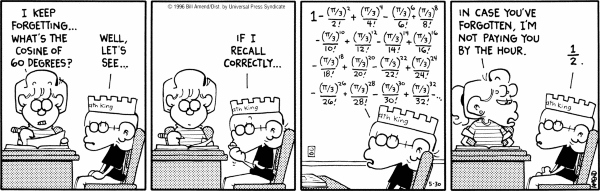
\includegraphics[width=0.618\textwidth]{pictures/taylor}
  \end{center}
\caption{MacLaurin-Reihe von $\cos(x)$}
\end{figure}
\begin{ueb}
Betrachte das Polynom $n$-ten Grades
$$f(x)=a_nx^n+a_{n-1}x^{n-1}+\dots+a_1x+a_0.$$
Notiere $f^{(k)}(0)$ f\"ur $k\in\set{0,\dots,n}$.
\end{ueb}
\noindent Daraus schliesst man, dass die Funktion $f$ in der Form
$$\frac{f^{(n)}(0)}{n!}x^n+\frac{f^{(n-1)}(0)}{(n-1)!}x^{n-1}+\dots+\frac{f'(0)}{1!}x+f(0)$$
dargestellt werden kann. Das heisst, dass sich die Funktion global durch die lokale Eigenschaft \glqq Ableitung bei $x=0$\grqq\ eindeutig festlegen l\"osst.
Da fast jede Funktion n\"oherungsweise als Reihe dargestellt werden kann, definiert man

\begin{defn}
Sei $f$ eine bei $x=0$ definierte und beliebig oft differenzierbare Funktion. Dann heisst das Polynom
$$T(x)=f(0)+\frac{f'(0)}{1!}x+\frac{f''(0)}{2!}x^2+\frac{f'''(0)}{3!}x^3+\dots$$
\textbf{MacLaurin-Reihe}.
Soll
\marginnote{
\qrcode{
https://www.youtube.com/watch?v=C5s-wQSWggY}
}
nicht zwangsl\"oufig um $x=0$ entwickelt werden, so spricht man allgemein von einer \textbf{Taylor-Reihe}.
\end{defn}

\begin{ueb}
Stellt jede Taylorreihe einer Funktion $f$ die Funktion auch selber dar? In andern Worten, konvergiert die Taylorreihe von $f$ gegen $f$?
\end{ueb}

\begin{bsp}
Wir betrachten einige Funktionen und deren Taylorentwicklung um $x=0$.
\begin{enumeratea}
\item F\"ur $f(x)=\sin(x)$ erhalten wir die bereits bekannte Darstellung
$$T(x)=x-\frac{x^3}{3!}+\frac{x^5}{5!}-\dots.$$
Es scheint so, als ob $\sin(x)$ als Taylorreihe darstellbar w\"ore.
\item $f(x)=\frac{1}{1-x}$ wird zu
$$T(x)=1+x+x^2+x^3+\dots,$$
was wir aus der Theorie \"uber Folgen \& Reihen kennen. Damit kann aber die Taylorentwicklung h\"ochstens f\"ur $-1<x<1$ gegen $f$ konvergieren.
\item Betrachten wir $f(x)=e^{-\frac{1}{x^2}}$ f\"ur $x\neq0$ mit seiner stetigen Fortsetzung $f(0)=0$, erhalten wir
$$T(x)=0.$$
Daher wird also $f$ nur in $x=0$ durch ihre Taylorreihe approximiert.
\end{enumeratea}
\end{bsp}

\begin{defn}
Eine Funktion $f$ heisst \textbf{analytisch}, falls sie in jedem Punkt durch eine konvergente Potenzreihe dargestellt werden kann.
\end{defn}
Zu den analytischen Funktionen geh\"oren die Polynome, die trigonometrischen und Exponentialfunktionen und deren Umkehrfunktionen, sowie die aus ihnen durch Grundrechenarten erzeugten Funktionen.
\begin{ueb}
Bestimme die Taylorreihen um $x=0$ der folgenden Funktionen.
\begin{enumeratea}
\item $f(x)=e^x$
\item $f(x)=\ln(1+x)$
\end{enumeratea}
\end{ueb}
F\"ur die Taylorentwicklung in einem Punkt $x_0\neq0$ einer Funktion $f$ findet man
$$T(x)=f(x_0)+f'(x_0)(x-x_0)+\frac{f''(x_0)}{2!}(x-x_0)^2+\dots$$
oder kurz
$$T_{x_0}(x)=\sum_{k=0}^\infty \frac{f^{(k)}(x_0)}{k!}(x-x_0)^k.$$
Damit kann $f$ st\"uckweise durch eine Taylorentwicklung an verschiedenen Stellen $x_0$ gut approximiert werden.
\begin{bem}
In vielen Belangen der Naturwissenschaften reicht ein Taylorpolynom recht niedrigen Grades zur Approximation von $f$ in einer gew\"ohlten Umgebung.
\end{bem} 

\begin{ueb}
Bestimme die Taylorentwicklung bei $x_0$ von
$$f(x)=\frac{1}{1-x}.$$
Berechne dazu zuerst $f^{(k)}(x)$. Notiere dann $T_{x_0}(x)$ in geschlossener Form und explizite die ersten drei Summanden. Berechne anschliessend N\"oherungen f\"ur z.B. $x_0=-2,0,2,\dots$.
\end{ueb}

\subsection{Rechnen mit Potenzreihen}

Schaut man sich die ersten vier nichtverschwindenden Terme der MacLaurin-Reihe von $\sin(x^2)$ an, so stellt man sich die Frage, ob diese Funktion nicht einfacher zu entwickeln w\"ore.

\begin{align*}
f(x) &= \sin(x^2) \\
f'(x) &= 2x\cos(x^2) \\
f''(x) &= 2\cos(x^2)-4x^2\sin(x^2) \\
f'''(x) &= -8x^3\cos(x^2)-12x\sin(x^2) \\
f^{(4)}(x) &= 16x^4\sin(x^2)-48x^2\cos(x^2)-12\sin(x^2)
\end{align*}
Somit $T(x)=x^2+\dots$ und die weiteren Terme sind m\"uhsam zu bestimmen. Einfacher geht es aber mit folgendem Satz.

\begin{satz}
Innerhalb des Konvergenzradius d\"urfen Potenzreihen addiert, subtrahiert, multipliziert und dividiert, gliedweise differenziert und integriert und in den Potenzreihen substituiert werden.
\end{satz}

\begin{bsp}
$$\sin(x^2)=x^2-\frac{x^6}{3!}+\frac{x^{10}}{5!}-\frac{x^{14}}{7!}+\dots$$
\end{bsp}

\begin{bsp}
\begin{align*}
\sin x\cdot\cos x &= \left(x-\frac{x^3}{3!}+\frac{x^5}{5!}+\frac{x^7}{7!}+\dots\right)
\cdot\left(1-\frac{x^2}{2!}+\frac{x^4}{4!}-\frac{x^6}{6!}+\dots\right)\\
 &= x-\left(\frac{1}{2!1!}+\frac{1}{3!}\right)x^3+
 +\left(\frac{1}{5!}+\frac{1}{4!1!}+\frac{1}{3!2!}\right)x^5-\dots\\
 &\stackrel{*}{=}x-\frac{4}{3!}x^3+\frac{16}{5!}x^5-\frac{64}{7!}x^7+\dots\\
 &=\frac{1}{2}\left(2x-\frac{(2x)^3}{3!}+\frac{(2x)^5}{5!}-\frac{(2x)^7}{7!}+\dots\right)\\
 &=\frac{1}{2}\sin(2x)
\end{align*}
Wir begr\"unden noch die Umformung bei $*$:
\begin{align*}
&\phantom{=}\frac{1}{(2k+1)!}+\frac{1}{(2k)!\cdot1!}+\frac{1}{(2k-1)!\cdot2!}
+\dots+\frac{1}{(k+1)!k!}\\
&=\frac{1+(2k+1)+\frac{(2k+1)2k}{2!}+\dots+\frac{(2k+1)!}{(k+1)!k!}}{(2k+1)!}\\
&=\frac{\binom{2k+1}{0}+\binom{2k+1}{1}+\dots+\binom{2k+1}{k+1}}{(2k+1)!}\\
&=\frac{2^{2k+1}/2}{(2k+1)!}\\
&=\frac{2^{2k}}{(2k+1)!}
\end{align*}
\end{bsp}

\begin{ueb}
Gib die ersten $4$ nicht verschwindenden Terme der MacLaurin-Reihe f\"ur
\begin{enumeratea}
\item $f(x)=\frac{x}{1-x^2}$
\item $g(x)=\frac{\ln(x+1)}{x}$
\item $h(x)=\ln(x)$
\end{enumeratea}
\end{ueb}

Ist eine Funktion $f$ durch ihre Taylorreihe darstellbar, so kann auf beiden Seiten der Gleichung abgeleitet oder integriert werden. Damit erh\"olt man neue Beziehungen.

\begin{bsp}
Sei
$$f(x)=\frac{1}{1-x}=1+x+x^2+x^3+\dots,$$
dann folgt bei Ableitung die aus der Wahrscheinlichkeitsrechnung bekannte \glqq Warten-auf-einen-Erfolg-Wahrscheinlichkeit\grqq
$$f'(x)=\frac{1}{(1-x)^2}=1+2x+3x^2+\dots.$$
Integriert man, so erscheint
$$\int f dx=-\ln(1-x)=x+\frac{1}{2}x^2+\frac{1}{3}x^3+\dots.$$
\end{bsp}

\begin{bem}
Als Z\"uckerchen erh\"alt man N\"aherungen f\"ur Stammfunktionen nicht geschlossen integrierbaren Funktionen wie zum Beispiel
$$
\int e^{x^2}dx =\int\left(1+x^2+\frac{x^4}{2!}+\dots\right)dx=x+\frac{1}{3}x^3+\frac{1}{10}x^5+\dots.
$$
\end{bem}

Nun ist auch klar, dass sich Taylorreihen eignen, um numerische L\"osungen von Differentialgleichungen zu finden. Wir verfolgen
\begin{bsp}
Betrachte
$$y''=y-x^3$$
mit den Anfangsbedingungen $f(0)=a_0=0$ und $f'(0)=a_1=6$. Wir w\"ahlen als Ansatz eine Potenzreihe
$$y=a_0+a_1x+a_2x^2+a_3x^3+\dots$$
mit zweiter Ableitung
$$y''=2a_2+6a_3x+12a_4x^2+20x^3+\dots.$$
Daraus erhalten wir
$$y-x^3=a_0+a_1x+a_2x^2+(a_3-1)x^3+\dots.$$
Es folgt
\begin{align*}
a_2&=\frac{1}{2}a_0, &a_3&=\frac{1}{6}a_1,\\
a_4&=\frac{1}{12}a_2=\frac{1}{24}a_0, &a_5&=\frac{1}{20}(\frac{1}{6}a_1-1)
\end{align*}
also
$$y=6x+x^3.$$
\end{bsp}

\begin{ueb}
L\"ose folgende Differentialgleichungen mit einem Potenzreihenansatz unter der Annahme, dass $x(t)$ bzw. $y(x)$ als Taylorreihe darstellbar ist.
\begin{enumeratea}
\item $\dot{x}=\ga x$
\item $\dot{x}=gt$
\item $\dot{x}=k\sqrt{x}$
\item $y''=\frac{6y-2}{x^2}+6x^2$
\item $y=xy'-x^2$ mit $y_0=0$
\end{enumeratea}
\end{ueb}

\subsection{Komplexe Exponentialfunktion}

Mit Hilfe der Taylorentwicklung f\"ur
$$e^x=\sum_{k=0}^\infty\frac{x^k}{k!}$$
m\"usste
\begin{align*}
e^{ix}&=\sum_{k=0}^\infty\frac{(ix)^k}{k!}\\
&=\sum_{k=0}^\infty\frac{(-1)^kx^{2k}}{(2k)!}+\sum_{k=0}^\infty\frac{(-1)^kx^{2k-1}}{(2k-1)!}\\
&=\cos x+i\sin x
\end{align*}
gelten. Und damit, man kann es nicht oft genug notieren,
$$e^{i\pi}+1=0.$$
Via
$$e^z=e^{a+ib}=e^a\cdot e^{ib}=e^a\cis b$$
erahnt man, dass die Ableitungsregeln f\"ur Exponentialfunktionen im Komplexen erhalten bleiben.

\subsection{Grenzwerte unbestimmter Ausdr\"ucke}

Taylorentwicklungen k\"onnen bei Grenzwert-Problemen helfen, wenn die direkte Berechnung auf Ausdr\"ucke der Art
$$\frac{0}{0}\q\text{oder}\q \frac{\pm\infty}{\pm\infty}$$
f\"uhrt.

\begin{bsp}
$$
\lim_{x\to0}\frac{\sin x}{x}=\lim_{x\to0}\frac{x-\frac{1}{3!}x^3+\frac{1}{5!}x^5-\dots}{x}=\lim_{x\to0}1-\frac{1}{3!}x^2+\frac{1}{5!}x^4-\dots=1
$$
\end{bsp}

\begin{ueb}
Bestimme
$$\lim_{x\to1}\frac{x-1}{\ln x}.$$
\end{ueb}

\noindent Allgemein ist diese Verfahrensweise bekannt unter dem Namen \glqq Regel von de L'Hospital\grqq.

\begin{satz}[Bernoulli-De L'Hospital]
Sei
\marginnote{
\qrcode{
https://www.youtube.com/watch?v=lRaQ7kAZTBs}
}
$$f(x)=\frac{z(x)}{n(x)}$$
mit $n,z$ differenzierbar und $n(x_0)=z(x_0)=0$ oder beide f\"ur $x\to x_0$ bestimmt divergent. Dann gilt
$$\lim_{x\to x_0}\frac{z(x)}{n(x)}=\lim_{x\to x_0}\frac{z'(x)}{n'(x)}.$$
\end{satz}

\begin{proof}
\"Ubung. Notiere die Taylorentwicklung von $n$ und $z$ bei $x_0$, falls $n(x_0)=z(x_0)=0$. F\"ur $n(x_0)=\pm\infty=z(x_0)$ betrachte man
$$f(x)=\frac{1/z(x)}{1/n(x)}.$$
\end{proof}

\begin{ueb}
Bestimme
\begin{enumeratea}
\item $\lim_{x\to0}x\ln x$
\item die Ableitung von $e^x$ mit Taylor
\item $\lim_{x\to0}x^x$ (Tipp: Schreibe als $e$-Funktion)
\item $\lim_{x\to0}\left(\frac{1}{x}-\frac{1}{\sin x}\right)$
\item $\lim_{x\to\infty}\frac{\ln(2x-1)}{e^x}$
\item $\lim_{x\to\infty}\sqrt{x}\ln x$
\item $\lim_{x\to\infty}\left(1+\frac{1}{x}\right)^x$
\end{enumeratea}
\end{ueb}

\section{Bogenl\"ange}

Zur Herleitung der Formel betrachten wir den Graphen einer im Intervall $[a,b]$ differenzierbaren Funktion $f$. Sei $L_a(x)$ die L\"ange des Bogens von der Stelle $a$ bis zur Stelle $x$; betrachte auch Abbildung \ref{abb:bogenlaenge} auf Seite \pageref{abb:bogenlaenge}.

\begin{figure}
\begin{center}
\definecolor{uququq}{rgb}{0.25,0.25,0.25}
\definecolor{xdxdff}{rgb}{0.49,0.49,1}
\scalebox{1.3}{
\begin{tikzpicture}[line cap=round,line join=round,>=triangle 45,x=0.95cm,y=1.0cm]
\draw[->,color=black] (-0.52,0) -- (6.82,0);
\foreach \x in {,1,2,3,4,5,6}
\draw[shift={(\x,0)},color=black] (0pt,2pt) -- (0pt,-2pt);
\draw[color=black] (6.48,0.08) node [anchor=south west] {$x$};
\draw[->,color=black] (0,-0.92) -- (0,4.56);
\foreach \y in {,1,2,3,4}
\draw[shift={(0,\y)},color=black] (2pt,0pt) -- (-2pt,0pt);
\draw[color=black] (0.1,4.16) node [anchor=west] {$y$};
\clip(-0.52,-0.92) rectangle (6.82,4.56);
\draw[smooth,samples=100,domain=1.1:6.8] plot(\x,{ln((\x)-1)+2});
\draw [dotted] (1.57,1.44)-- (1.57,0);
\draw [dotted] (2.74,0)-- (2.74,2.55);
\draw [dotted] (4.71,3.31)-- (4.71,0);
\draw (2.74,2.55)-- (4.71,2.55);
\draw (2.74,2.55)-- (4.71,3.31);
\draw (4.71,3.31)-- (4.71,2.55);
\draw (3.54,2.5) node[anchor=north west] {$ \Delta x $};
\draw (4.7,3.2) node[anchor=north west] {$ \Delta y $};
\begin{scriptsize}
\fill [color=xdxdff] (1.57,0) circle (1.5pt);
\draw[color=xdxdff] (1.58,-0.24) node {$a$};
\fill [color=xdxdff] (2.74,0) circle (1.5pt);
\draw[color=xdxdff] (2.72,-0.24) node {$x$};
\fill [color=xdxdff] (4.71,0) circle (1.5pt);
\draw[color=xdxdff] (4.7,-0.24) node {$x+\Delta x$};
\fill [color=xdxdff] (5.7,0) circle (1.5pt);
\draw[color=xdxdff] (5.7,-0.24) node {$b$};
\fill [color=uququq] (1.57,1.44) circle (1.5pt);
\draw[color=uququq] (1.38,1.72) node {$A$};
\fill [color=uququq] (2.74,2.55) circle (1.5pt);
\draw[color=uququq] (2.5,2.7) node {$P$};
\fill [color=uququq] (4.71,3.31) circle (1.5pt);
\draw[color=uququq] (4.64,3.6) node {$Q$};
\end{scriptsize}
\end{tikzpicture}
}
\end{center}
\caption{Illustration der Bogenl\"ange einer Funktion $f$}\label{abb:bogenlaenge}
\end{figure}

Dann ist $\hat{AQ}=L_a(x+\Delta x)$ und $\hat{PQ}=\hat{AQ}-\hat{AP}=L_a(x+\Delta x)-L_a(x)$. Aus der Graphik erkennt man $\overline{PQ}\leq\hat{PQ}$. Mit Hilfe des Satzes von Pythagoras folgt
$$
\overline{PQ} =\sqrt{\Delta x^2+\Delta y^2}=\sqrt{\Delta x^2\left(1+\frac{\Delta y^2}{\Delta x^2}\right)}=\Delta x\sqrt{1+\frac{\Delta y^2}{\Delta x^2}}
$$
Daraus folgt
$$\Delta x\sqrt{1+\frac{\Delta y^2}{\Delta x^2}}\leq L_a(x+\Delta x)-L_a(x)$$
und nach Division mit $\Delta x$
$$\sqrt{1+\frac{\Delta y^2}{\Delta x^2}}\leq\frac{L_a(x+\Delta x)-L_a(x)}{\Delta x}.$$
Nun lassen wir $Q$ gegen $P$ gehen:
$$\lim_{\Delta x\to0}\frac{\Delta y^2}{\Delta x^2}=f'(x)^2$$
und
$$\lim_{\Delta x\to0}\frac{L_a(x+\Delta x)-L_a(x)}{\Delta x}=L_a'(x)$$
wobei nun Gleichheit f\"ur die L\"angen gilt,  $\overline{PQ}=\hat{PQ}$.
Nun muss man noch eine Stammfunktion f\"ur $\sqrt{1+f'(x)^2}$ finden, dann haben wir auch $L_a(x)$. Somit folgt f\"ur die Bogenl\"ange entlang $f$ von $a$ nach $b$
$$L_a(b)=\int_a^b\sqrt{1+f'(x)^2}dx.$$
\begin{bem}
An $f$ muss zus\"atzlich zur Differenzierbarkeit auf $(a,b)$ auch noch die Stetigkeit der Ableitung vorausgesetzt werden.
\end{bem}

\section{Schwingungen}
\subsection{Freie unged\"ampfte Schwingung}

\begin{wrapfigure}{r}{0.382\textwidth}
\vspace{20pt}
  \begin{center}
    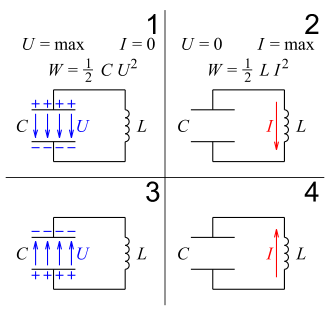
\includegraphics[width=0.382\textwidth]{pictures/schwing}
  \end{center}
\caption{Schwingungen}
\vspace{-50pt}
\end{wrapfigure}

F\"ur
\marginnote{
\qrcode{
https://www.youtube.com/watch?v=KEgk-5s7VVM}
}
die Auslenkung eines Massenpunktes $m$ gilt nach dem Hook'schen Gesetz
$$F=-k_0x$$
wobei $k_0$ die Federkonstante bezeichnet. Die Bewegungsgleichung lautet daher
\begin{align*}
ma &= -k_0x\\
m\ddot{x} &= -k_0x
\end{align*}
was wir mit $\go_0^2=\frac{k_0}{m}$ in der Form
$$\ddot{x}+\go_0^2 x=0$$
schreiben. Als L\"osungsansatz w\"ahlen wir
$$x(t)=Ce^{\gl t}.$$
Eingesetzt ergibt dies $\gl^2+\go_0^2=0$ und damit
$$\gl_{1,2}=\pm i\go_0.$$
Wir erhalten also die beiden L\"osungen
\begin{align*}
x_1(t) &= C_1e^{i\go_0 t}\\
x_2(t) &= C_2e^{-i\go_0 t},
\end{align*}
die f\"ur $\go_0\neq0$ linear unabh\"angig sind. Die allgemeine L\"osung der Differentialgleichung ist dann eine Linearkombination
$$x(t)=C_1e^{i\go_0 t}+ C_2e^{-i\go_0 t}.$$
Da $x(t)$ eine \emph{reelle} Funktion sein muss, impliziert das f\"ur komplexe Konstanten $C_1=C_2^*$. Wir setzen $C_1=a+ib$ und $C_2=a-ib$ und erhalten mit der Euler'schen Formel die allgemeine L\"osung
$$x(t)=2a\cos(\go_0 t)-2b\sin(\go_0 t)$$
oder k\"urzer
$$x(t)=k_1\cos(\go_0 t)+k_2\sin(\go_0 t).$$
Unter Kenntnis des Additionstheorems
$$\sin(x+y)=\sin x\cos y+\sin y\cos x$$
l\"asst sich $k_1$ als $x_0\sin\varphi$ und $k_2$ als $x_0\cos\varphi$ auffassen, was
$$x(t)=x_0\sin(\go_0 t+\varphi)$$
liefert.

\begin{figure}
\begin{center}
\definecolor{cqcqcq}{rgb}{0.75,0.75,0.75}
\scalebox{1.5}{
\begin{tikzpicture}[line cap=round,line join=round,>=triangle 45,x=0.8cm,y=1.0cm]
\draw [color=cqcqcq,dash pattern=on 1pt off 1pt, xstep=1.2566370614359172cm,ystep=1.0cm] (-0.96,-1.32) grid (7.74,1.24);
\draw[->,color=black] (-0.96,0) -- (7.74,0);
\foreach \x in {0.5,1,1.5,2}
\draw[shift={(\x*3.14,0)},color=black] (0pt,2pt) -- (0pt,-2pt) node[below] {\footnotesize $\x\pi$};
\draw[color=black] (7.5,0.03) node [anchor=south west] {$x$};
\draw[->,color=black] (0,-1.32) -- (0,1.24);
\foreach \y in {-1,1}
\draw[shift={(0,\y)},color=black] (2pt,0pt) -- (-2pt,0pt) node[left] {\footnotesize $\y$};
\draw[color=black] (0.07,1.11) node [anchor=west] {$y$};
\clip(-0.96,-1.32) rectangle (7.74,1.24);
\draw[smooth,samples=100,domain=-0.9570994940978063:7.741433389544653] plot(\x,{sin(((\x)+0.76)*180/pi)});
\end{tikzpicture}
}
\end{center}
\caption{Freie un\-ge\-d\"ampf\-te Schwingung}
\end{figure}

\subsection{Freie ged\"ampfte Schwingung}

Wie im vorangegangenen Kapitel betrachten wir eine Federschwingung; jetzt aber
\marginnote{
\qrcode{
https://www.youtube.com/watch?v=eXkSAAYvprc}
}
ged\"ampft durch eine Kraft, die wir proportional zur Geschwindigkeit des Massenpunktes annehmen. Dies beobachtet man zum Beispiel bei einer laminaren Str\"omung eines Mediums um den schwingenden K\"orper. Die Bewegungsgleichung lautet jetzt
$$ma=-k_0x-\gb \dot{x}.$$
Umschreiben:
\begin{align*}
m\ddot{x}+\gb \dot{x}+k_0x &=0\\
\ddot{x} +\frac{\gb}{m}\dot{x}+\frac{k_0}{m}x&=0\\
\ddot{x}+2k\dot{x}+\go_0^2 x &=0
\end{align*}
mit $\frac{\gb}{m}=2k$ und $\frac{k_0}{m}=\go_0^2$.
Im Falle $k\geq0$ und $\go_0^2\geq0$ w\"ahlen wir den L\"osungsansatz
$$x(t)=Ce^{\gl t}.$$
Eingesetzt ergibt sich die charakteristische Gleichung
$$\gl^2+2k\gl+\go_0^2=0$$
mit der L\"osung
$$\gl_{1,2}=-k\pm\sqrt{k^2-\go_0^2}.$$
Wegen der Pr\"asenz von zwei Variablen, $k$ und $\go_0$, m\"ussen wir verschiedene F\"alle unterscheiden.

\begin{description}
\item[Fall 1] Ist $k>\go_0$, so haben wir starke D\"ampfung; der sogenannte \emph{Kriechfall}. $\gl_1$ und $\gl_2$ sind somit reell und voneinander verschieden. Die L\"osung in diesem Fall ist
$$x(t)=k_1e^{\gl_1 t}+k_2e^{\gl_2 t}.$$

F\"ur $k_1=20, k_2=-20,\gl_1=-0.5$ und $\gl_2=-2.5$ ergibt sich folgendes Bild.

\begin{figure}
\begin{center}
\definecolor{cqcqcq}{rgb}{0.75,0.75,0.75}
\scalebox{1.2}{
\begin{tikzpicture}[line cap=round,line join=round,>=triangle 45,x=1.0cm,y=0.5cm]
\draw [color=cqcqcq,dash pattern=on 3pt off 3pt, xstep=1.57cm,ystep=1.0cm] (0,-1) grid (6.5,11);
\draw[->,color=black] (-0.5,0) -- (6.5,0);
\foreach \x in {0.5,1,1.5,2}
\draw[shift={(\x*3.14,0)},color=black] (0pt,2pt) -- (0pt,-2pt) node[below] {\footnotesize $\x\pi$};
\draw[color=black] (6.31,0.16) node [anchor=south west] { x};
\draw[->,color=black] (0,-2) -- (0,12);
\foreach \y in {2,4,6,8,10}
\draw[shift={(0,\y)},color=black] (2pt,0pt) -- (-2pt,0pt) node[left] {\footnotesize $\y$};
\draw[color=black] (0.05,11.21) node [anchor=west] { y};
\clip(-0.5,-2) rectangle (6.5,12);
\draw plot[raw gnuplot, id=func0] function{set samples 100; set xrange [0:6.4]; plot 20*2.71**(-0.5*x)-20*2.71**(-2.5*x)};
\end{tikzpicture}
}
\end{center}
\caption{Freie ged\"ampfte Schwingung: Kriech\-fall}
\end{figure}

\item[Fall 2] Mit $k=\go_0$ erreicht man starke D\"ampfung,  der sogenannte \emph{aperiodische Grenzfall}; $\gl_1=\gl_2=-k<0$.
Als L\"osung erhalten wir damit
$$x(t)=k_1e^{-kt}+k_2te^{-kt}.$$
Der Bewegungsablauf gleicht also dem vom Fall 1. In diesem Fall kommen schwingf\"ahige Systeme am schnellsten zur Ruhe, was zum Beispiel bei der Konstruktion von Messger\"aten/Zeigerinstrumenten erreicht werden will. Unten ist der Verlauf f\"ur $k_1=0, k_2=10$ und $k=-2.5$ illustriert.

\begin{figure}
\begin{center}
\definecolor{cqcqcq}{rgb}{0.75,0.75,0.75}
\scalebox{1.5}{
\begin{tikzpicture}[line cap=round,line join=round,>=triangle 45,x=1.0cm,y=1.5cm]
\draw [color=cqcqcq,dash pattern=on 1pt off 1pt, xstep=1.57cm,ystep=0.75cm] (0,0) grid (6.5,1.7);
\draw[->,color=black] (-0.5,0) -- (6.5,0);
\foreach \x in {0.5,1,1.5,2}
\draw[shift={(\x*3.14,0)},color=black] (0pt,2pt) -- (0pt,-2pt) node[below] {\footnotesize $\x\pi$};
\draw[color=black] (6.23,0.03) node [anchor=south west] {$\go t$};
\draw[->,color=black] (0,-0.5) -- (0,2);
\foreach \y in {0.5,1,1.5}
\draw[shift={(0,\y)},color=black] (2pt,0pt) -- (-2pt,0pt) node[left] {\footnotesize $\y$};
\draw[color=black] (0.05,1.86) node [anchor=west] {$x(t)$};
\clip(-0.5,-0.5) rectangle (6.5,2);
\draw plot[raw gnuplot, id=func0] function{set samples 100; set xrange [0:6.4]; plot 10*x*2.71**(-2.5*x)};
\end{tikzpicture}
}
\end{center}
\caption{Freie ged\"ampfte Schwingung: aperiodischer Grenzfall}
\end{figure}

\item[Fall 3] Schwache D\"ampfung, einen sogenannten \emph{Schwingfall}, erh\"alt man f\"ur $k<\go_0$.
Dabei sind $\gl_1$ und $\gl_2$ konjugiert komplexe Wurzeln, $\gl_{1,2}=-k\pm\go_1i$ mit $\go_1=\sqrt{\go_0^2-k^2}$. Die L\"osung ist
$$x(t)=e^{-kt}(k_1\cos(\go_1 t)+k_2\sin(\go_1 t))$$
oder, \"ahnlich der Behandlung freier Schwingungen mittels Additionstheorem,
$$x(t)=Ae^{-kt}\sin(\go_1 t+\varphi),$$
mit $A^2=k_1^2+k_2^2$ und $\tan\varphi=\frac{k_1}{k_2}$. Dies ist die ged\"ampfte harmonische Schwingung; es folgt $T>T_0$.

$\go_1=\sqrt{\go_0^2-k^2}$ zeigt, dass im Falle der ged\"ampften Schwingung die Kreisfrequenz $\go_1$ kleiner als die Kreisfrequenz $\go_0$ der freien Schwingung ist. Charakterisiert wird das Verhalten der ged\"ampften Schwingung durch das Verh\"altnis zweier aufeinanderfolgender, gleichgerichteter Amplituden:
$$\frac{x_n}{x_{n+1}}=\frac{x(t_0)}{x(t_0+T)}=e^{kT}$$
mit dem sogenannten logarithmischen Dekreten $\gL=kT$.

\begin{figure}
\begin{center}
\definecolor{cqcqcq}{rgb}{0.75,0.75,0.75}
\scalebox{1.5}{
\begin{tikzpicture}[line cap=round,line join=round,>=triangle 45,x=0.2cm,y=2.0cm]
\draw [color=cqcqcq,dash pattern=on 2pt off 2pt, xstep=0.3141592653589793cm,ystep=1.0cm] (-3,-1.2) grid (25.5,1.2);
\draw[->,color=black] (-3,0) -- (25.5,0);
\foreach \x in {-1.57,1.57,3.15,4.71,6.28,7.85,9.42,11,12.57,14.14,15.71,17.28,18.85,20.42,21.99,23.56,25.13}
\draw[shift={(\x,0)},color=black] (0pt,2pt) -- (0pt,-2pt);
\draw[color=black] (24.38,0.03) node [anchor=south west] { $\go t$};
\draw[->,color=black] (0,-1.2) -- (0,1.2);
\foreach \y in {-1,-0.5,0.5,1}
\draw[shift={(0,\y)},color=black] (2pt,0pt) -- (-2pt,0pt) node[left] {\footnotesize $\y$};
\draw[color=black] (0.22,1.06) node [anchor=west] { $x(t)$};
\clip(-3,-1.2) rectangle (25.5,1.2);
\draw plot[raw gnuplot, id=func3] function{set samples 100; set xrange [0.1:25.1]; plot 2.71**(-0.1*x)*sin((3.14/180*x)*180/3.14)};
\draw[dash pattern=on 2pt off 2pt] plot[raw gnuplot, id=func4] function{set samples 100; set xrange [0.1:25.1]; plot 2.71**(-0.1*x)};
\draw[dash pattern=on 2pt off 2pt] plot[raw gnuplot, id=func5] function{set samples 100; set xrange [0.1:25.1]; plot -2.71**(-0.1*x)};
\end{tikzpicture}
}
\end{center}
\caption{Ged\"ampfte harmonische Schwingung}
\end{figure}
\end{description}


\subsection{Erzwungene Schwingung}
Wir
\marginnote{
\qrcode{
https://www.youtube.com/watch?v=3zc1PeyGRAY}
}
betrachten eine ged\"ampfte Schwingung, die periodisch mit der Kraft $F=ma_0\cos(\go t)$ angetrieben wird. Die Schwingungsgleichung lautet
$$\ddot{x}+2k\dot{x}+\go_0^2x=a_0\cos(\go t).$$
Dies ist eine inhomogene lineare Differentialgleichung zweiter Ordnung. Zur L\"osung kommen wir wie gelernt
\begin{enumeratea}
\item l\"osen der homogenen Gleichung
\item erg\"anzen der L\"osung mit einer partikul\"aren
\end{enumeratea}
Die homogene Differentialgleichung wurde im Kapitel zur freien, ged\"ampften Schwingung hergeleitet. F\"ur geringe D\"ampfung ergab sich --- wenn wir nur den homogenen Teil benutzen ---
$$x_{hom}=Ae^{-kt}\sin(\go_1 t+\varphi)$$
mit $\go_1=\sqrt{\go_0^2-k^2}$.

Um die allgemeine L\"osung zu gewinnen, bleibt eine partikul\"are L\"osung der inhomogenen Differentialgleichung zu bestimmen. Als Ausgangspunkt daf\"ur nutzen wir eine experimentelle Beobachtung: Das System schwingt demnach immer mit der Erregerfrequenz $\go$, die Eigenfrequenz $\go_1$ spielt mit der Zeit keine Rolle. Daher w\"ahlen wir den L\"osungsansatz
$$x_{part}=a\sin(\go t)+b\cos(\go t).$$
Wir kommen mit einer einfachen Rechnung zum Ziel, wenn wir einen komplexen Ansatz w\"ahlen. Wegen $a_0\cos(\go t)=\re(a_0e^{i\go t})$ w\"ahlen wir
$$x_{part}=Ce^{i\go t}.$$
Damit ergibt sich der komplexe Ansatz
$$-\go^2Ce^{i\go t}+2ki\go Ce^{i\go t}+\go_0^2Ce^{i\go t}=a_0e^{i\go t}.$$
Das heisst $C(\go_0^2-\go^2+2ik\go)=a_0$. Zur Analyse unterscheidet man zwei F\"alle --- Klammerausdruck gleich oder ungleich $0$.

\begin{description}
\item[Fall 1] Sei $\go_0^2-\go^2+2ik\go\neq0$, das heisst $\re(\go_0^2-\go^2)\neq0$ oder $\im(2ik\go)\neq0$. Somit
$$C=\frac{a_0}{\go_0^2-\go^2+i\cdot 2k\go},$$
was komplex erweitert
$$
C=\frac{a_0(\go_0^2-\go^2)}{(\go_0^2-\go^2)^2+4k^2\go^2}-i\frac{2k\go a_0}{(\go_0^2-\go^2)^2+4k^2\go^2}
$$
ergibt. Damit erhalten wir f\"ur unseren Ansatz
$$
\re(Ce^{i\go t})=\frac{a_0(\go_0^2-\go^2)}{(\go_0^2-\go^2)^2+4k^2\go^2}\cos(\go t)+\frac{2k\go a_0}{(\go_0^2-\go^2)^2+4k^2\go^2}\sin(\go t).
$$
Eine weitere Vereinfachung mittels des Additionstheorems
$$\cos(x+y)=\cos x\cos y-\sin x\sin y$$
kann vorgenommen werden, wenn man den Faktor
$$\frac{a_0}{\sqrt{(\go_0^2-\go^2)^2+4k^2\go^2}}$$
ausklammert. Erst dann l\"asst sich die f\"ur die Winkelfunktion notwendige Bedingung $\sin^2x+\cos^2x=1$ erf\"ullen. Es folgt
$$
\re(Ce^{i\go t})=\frac{a_0}{\sqrt{(\go_0^2-\go^2)^2+4k^2\go^2}}\cdot(\cos\ga\cos(\go t)-\sin\ga\sin(\go t))
$$
mit
$$\cos\ga=\frac{(\go_0^2-\go^2)}{\sqrt{(\go_0^2-\go^2)^2+4k^2\go^2}}$$
und
$$\sin\ga=-\frac{2k\go}{\sqrt{(\go_0^2-\go^2)^2+4k^2\go^2}}.$$
Wir haben endlich
\begin{align*}
x_{part}&=\re(Ce^{i\go t})\\
&=\frac{a_0}{\sqrt{(\go_0^2-\go^2)^2+4k^2\go^2}}\cos(\go t+\ga)
\end{align*}
mit $\tan\ga=-\frac{2k\go}{\go_0^2-\go^2}$ und damit f\"ur die L\"osungsgesamtheit die allgemeine L\"osung
$$
x(t)=Ae^{-kt}\sin(\go_1 t+\varphi)+\frac{a_0}{\sqrt{(\go_0^2-\go^2)^2+4k^2\go^2}}\cos(\go t+\ga)
$$

\begin{bem}
F\"ur grosse Zeiten strebt der Anteil der homogenen L\"osung gegen Null. Das bedeutet, dass im station\"aren Zustand das Verhalten des Systems durch die partikul\"are L\"osung bestimmt ist.
\end{bem}

\item[Fall 2] Man erh\"alt f\"ur $\go_0^2=\go^2$ mit $k=0$ Resonanz. Wegen des Anwachsens der Amplitude versucht man einen partikul\"aren Ansatz mit Wachstum,
$$x_{part}=Cte^{i\go_0 t}.$$
Nach Einsetzen folgt
$$2Ci\go_0=a_0$$
oder
$$C=-\frac{a_0}{2\go_0}i.$$
Wir erhalten
$$x_{part}=\re(Cte^{i\go_0 t})=\frac{a_0}{2\go_0}t\sin(\go_0 t)$$
und f\"ur die L\"osungsgesamtheit
$$
x(t)=\frac{a_0}{2\go_0}t\sin(\go_0 t)+k_1\cos(\go_0 t)+k_2\sin(\go_0 t).
$$
\begin{bem}
Hier sorgt der partikul\"are L\"osungsanteil f\"ur grosse Ausschl\"age, die man im Resonanzfall erwartet.
\end{bem}
\end{description}

\clearpage

\appendix

\section{Numerische Verfahren}
\begin{wrapfigure}{r}{0.382\textwidth}
  \begin{center}
    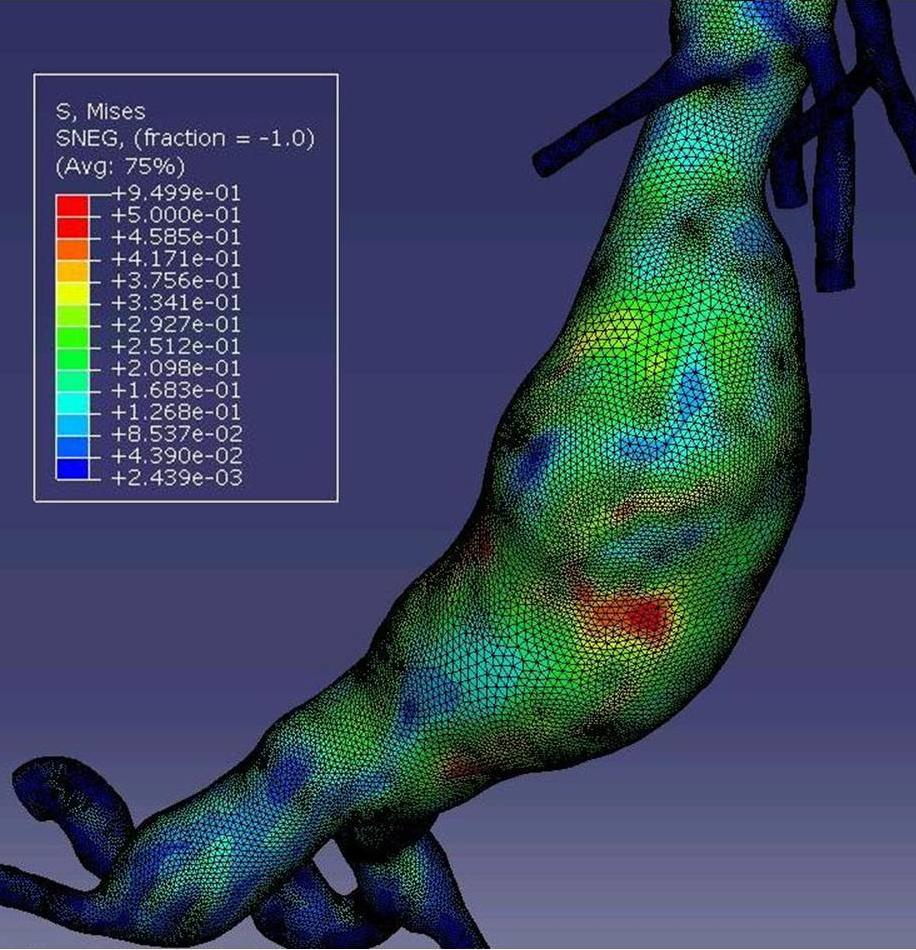
\includegraphics[width=0.382\textwidth]{pictures/aneurysma}
  \end{center}
%\caption{A gull}
\end{wrapfigure}
Um L\"osungen zu Differentialgleichungen zu finden, Trajektorien und zeitabh\"angige Graphen zu plotten, sind wir auf die Hilfe von leistungsstarken Computern und Software angewiesen. Einige Packages, wie zum Beispiel \texttt{Mathematica}, liefern wenn immer m\"oglich analytische L\"osungen. Viele Probleme jedoch k\"onnen nicht analytisch gel\"ost werden. Deshalb interessieren numerische Verfahren, die N\"aherungsl\"osungen liefern. Diese wiederum sollten nat\"urlich m\"oglichst nahe an die exakte L\"osung kommen.

Einige gewichtige Nachteile treten bei computergenerierten L\"osungen auf, insbesondere falls die L\"osungen numerisch berechnet werden. M\"ogliche Fehler sind

\begin{itemize}
\item Rundungsfehler, die mit steigender Anzahl Berechnungen zunehmen.
\item Diskretisierungsfehler, verursacht durch die Einschr\"ankung auf eine Teilmenge bzw. eine endliche Anzahl von Punkten.
\item Durch das verwendete N\"aherungsverfahren verursachte Abweichungen von der exakten L\"osung.
\end{itemize}

Es gibt zahlreiche numerische Verfahren zur Bestimmung von Ableitungen, Integralen, Summen etc. Wir wollen uns im Folgenden einen Auszug aus der Vielfalt der Verfahren anschauen und kurz auf deren Genauigkeit absch\"atzen.

\subsection{Numerische Standardverfahren}

Wir betrachten eine Differentialgleichung der Form
$$y'=f(t,y)$$
mit Startwert $y_0=y(t_0)$ und wenden darauf die folgenden Verfahren an, um $y(t)$ \"uber einem Zeitintervall $t_0<t<T$ numerisch abzusch\"atzen.

Wir beginnen mit einer simplen Methode, dem Euler-Verfahren, um die grunds\"atzliche Idee eines N\"aherungsverfahren zu erfassen und besprechen dann eine weit verbreitete Methode, das Runge-Kutta-Verfahren.

\subsubsection{Das Euler-Verfahren}

Klar ist, dass ein Computer nicht jeden Punkt einer Kurve berechnen kann, weil es ja unendlich viele davon gibt. Also beschr\"ankt sich ein N\"aherungsverfahren immer auf eine diskrete Teilmenge. Euler's Methode beschreibt eine sehr einfache Ann\"aherung an die L\"osung einer Differentialgleichung f\"ur eine endliche Anzahl von Punkten. Die Teilschritte sind

\begin{enumerate}
\item Teile das betrachtete Intervall in $N$ gleich grosse Abschnitte und setze f\"ur $n=0,1,2,\dots,N-1$
$$t_n=t_0+nh,$$
wobei $h=\frac{T-t_0}{N}$ die Schrittweite ist.
\item Ausgehend vom Punkt $\point{t_0}{y_0}$ auf der Kurve approximiert man $y_n=y(t_n)$. Eine N\"aherung f\"ur $y_1$ bestimmen wir via der Tangente durch $\point{t_0}{y_0}$ bis $t_1$. Also
$$y_1\approx y_0+hf(t_0,y_0)$$
mit
$$y'=f(t_0,y_0)\approx\frac{y_1-y_0}{h}=\frac{y_1-y_0}{t_1-t_0}.$$
\item Bestimme so $y_2\approx y_1+f(t_1,y_1)$ und weiter $y_3,\dots,y_n$.
\end{enumerate}

Allgemein beschrieben hat man das rekursive Schema
$$y_{n+1}=y_n+hf(t_n,y_n)$$
mit
$$t_{n+1}=t_n+h$$
f\"ur $0\leq n\leq N-1$.

\begin{figure}
\begin{center}
\scalebox{1.3}{
\begin{tikzpicture}[line cap=round,line join=round,>=triangle 45,x=0.82cm,y=0.82cm]
\draw[->,color=black] (-0.88,0) -- (7.62,0);
\foreach \x in {,1,2,3,4,5,6,7}
\draw[shift={(\x,0)},color=black] (0pt,-2pt);
\draw[color=black] (7.34,0.08) node [anchor=south west] {$t$};
\draw[->,color=black] (0,-1.2) -- (0,4.44);
\foreach \y in {-1,1,2,3,4}
%\draw[shift={(0,\y)},color=black] (2pt,0pt) -- (-2pt,0pt);
\draw[color=black] (0.1,4.04) node [anchor=west] {$y$};
\clip(-0.88,-1.2) rectangle (7.62,4.44);
\draw plot[raw gnuplot, id=func0] function{set samples 100; set xrange [0:2]; plot 1};
\draw plot[raw gnuplot, id=func1] function{set samples 100; set xrange [2:4]; plot 0.2*x+0.6};
\draw plot[raw gnuplot, id=func2] function{set samples 100; set xrange [4:6]; plot 0.4*x-0.2};
\draw plot[raw gnuplot, id=func3] function{set samples 100; set xrange [6:7]; plot 0.6*x-1.4};
\draw plot[raw gnuplot, id=func4] function{set samples 100; set xrange [0:7]; plot 0.05*x**2+1};
\draw (3.36,2.82) node[anchor=north west] {L\"osung};
\draw (5.62,2.1) node[anchor=north west] {Euler};
\draw (-0.8,1.38) node[anchor=north west] {$y_0$};
\draw (0.06,0) node[anchor=north west] {$t_0$};
\draw (2.06,0) node[anchor=north west] {$t_1$};
\draw (4.06,0) node[anchor=north west] {$t_2$};
\draw (6.06,0) node[anchor=north west] {$t_3$};
\end{tikzpicture}
}
\end{center}
\caption{Das Euler-Verfahren}
\end{figure}

\begin{bsp}
Wir bestimmen mit dem Euler-Verfahren mit Schrittweite $h=0.1$ eine N\"aherung f\"ur $y(0.2)$ der Gleichung
$$\frac{dy}{dt}=y^2+t$$
mit Startwert $y(0)=1$.

Hier ist $f(t,y)=y^2+t$. F\"ur $n=0$ ist
$$y_1=y(0.1)=y_0+hf(t_0,y_0)=1.1.$$
Mit $n=1$ erhalten wir
$$y_2=y(0.2)=y_1+hf(t_1,y_1)=1.231.$$
\end{bsp}

\begin{ueb}
Rechne $y_1$ und $y_2$ aus obigem Beispiel nach.
\end{ueb}

Vergleichen wir die Taylor-Entwicklung von
$$y_{n+1}=y_n+h\frac{dy_n}{dt}+\frac{h^2}{2!}\frac{d^2y_n}{dt^2}+\dots$$
mit der Euler-Methode, so sehen wir, dass letztere aus den ersten zwei Summanden besteht. Man sagt: Das Euler-Verfahren ist eine first-order Approximation. Nun versuchen wir aufgrund dieser Beobachtung den Fehler abzusch\"atzen und m\"oglicherweise durch Anpassung der Schrittweite den Fehler zu kontrollieren.

Euler liefert den N\"aherungswert
$$y_{n+1}=y_n+hf(t_n,y_n)$$
und Taylor den wahren Wert
$$y(t_{n+1})=y(t_n)+hf(t_n,y(t_n))+\frac{h^2}{2}f'(\gz,y(\gz_n))$$
wobei $\gz_n$ zwischen $t_n$ und $t_{n+1}$ liegt. Subtrahieren wir Euler von Taylor erhalten wir den Fehlerterm
$$
E_{n+1}=y(t_n)-y_n+
h(f(t_n,y(t_n))-f(t_n,y_n))+\frac{h^2}{2}f'(\gz_n,y(\gz_n)).
$$
Man kann zeigen, dass dieser Fehlerterm durch
$$E_{n+1}\leq \frac{Dh}{2L}(e^{T-t_0}-1)$$
nach oben beschr\"ankt ist, wobei $L$ eine obere Schranke f\"ur $f$ und $D$ eine obere Schranke f\"ur $f'$ \"uber dem Intervall $[t_0,T]$ ist und $f$ gutm\"utig sowie $T=t_0+(N-1)h$.

Wegen $\lim_{h\to0}E_{n+1}=0$ liegt die Vermutung nahe, dass die Genauigkeit mit kleiner werdenden Schrittweite zunimmt; was auch bewiesen wurde. Aber, da eine kleinere Schrittweite mit mehr Berechnungen einhergeht, und der Computer dabei \"ofter Runden muss, nehmen diese Rundungsfehler zu. Um das beste Resultat zu erzielen sollten wir also ein Optimum f\"ur die Schrittweite finden, so dass die Kombination der beiden Fehler minimiert wird.

\subsubsection{Das Runge-Kutta-Verfahren}

One-step Algorithmen, die durchschnittliche Steigungen einer Funktion $f(t,y)$ in zwei oder mehreren Punkten \"uber einem Intervall $[t_{n-1},t_n]$ verwenden um $y_n$ zu berechnen, heissen \textbf{Runge-Kutta Methoden}. Sie sind auch charakteristisch f\"ur sogenannte \emph{predictor-corrector} Methoden, weil sie eine Vorhersage f\"ur folgende Werte geben und danach mit einer Serie von Gewichten diese Werte korrigieren.

Eine weit verbreitete Methode ist das Runge-Kutta-Verfahren vierter Ordnung (RK4). Es verwendet gewichtete durchschnittliche Steigungen um die Mittel- und Endpunkte von Teilintervallen. Algorithmisch formuliert
$$y_{n+1}=y_n+\frac{h}{6}(k_1+2k_2+2k_3+k_4)$$
mit
\begin{align*}
k_1 &= f(t_n,y_n)\\
k_2 &= f(t_n+\frac{h}{2},y_n+\frac{h}{2}k_1)\\
k_3 &= f(t_n+\frac{h}{2},y_n+\frac{h}{2}k_2)\\
k_4 &= f(t_n+h,y_n+hk_3)
\end{align*}

Eine weitere Runge-Kutta Methode mit einem einfacheren Prinzip der Mitteilung ist das \textbf{Heun's-Verfahren}. Wie das Euler-Verfahren ist es ein one-step Algorithmus, aber es ist genauer:
$$y_{n+1}=y_n+\frac{h}{2}(k_1+k_2)$$
mit
\begin{align*}
k_1 &= f(t_n,y_n)\\
k_2 &= f(t_n+h,y_n+hk_1)
\end{align*}

\begin{ueb}
Zeichne eine Illustration zum Heun-Verfahren.
\end{ueb}

\newpage

\section{Ein Raketenmodell}
\begin{figure}
  \begin{center}
    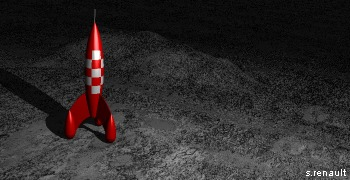
\includegraphics[width=0.618\textwidth]{pictures/raketetim}
  \end{center}
%\caption{A gull}
\end{figure}

Wir betrachten das klassische \glqq Pfupfmodel\grqq\ einer Rakete der Masse $m$ mit Geschwindigkeit $v$ und verwenden den Impulserhaltungssatz. Also notieren wir jeweils den Impuls $p$ vor und nach dem \glqq Stoss\grqq\ und vergleichen.

\begin{figure}[h!]
  \begin{center}
    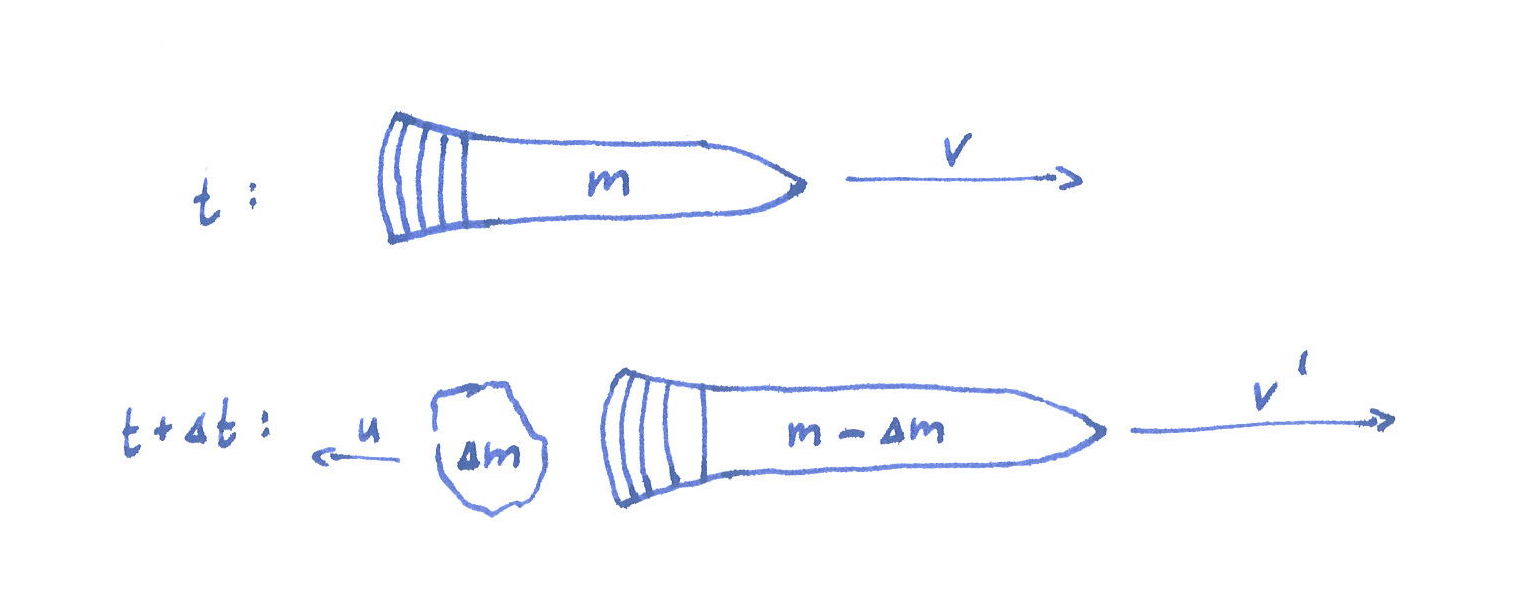
\includegraphics[width=0.618\textwidth]{pictures/raketeimpuls}
  \end{center}
\caption{Pfupf-Modell einer Rakete}
\end{figure}

Mit obiger Notation gilt:
$$p=(m-\gD m)\cdot v'+\gD m\cdot(v'-u)$$
und unmittelbar folgt f\"ur $p=mv$
$$mv=mv'-\gD mu$$
wobei $v'$ die Geschwindigkeit der Rakete nach dem Stoss und $u$ die Ausstr\"omgeschwindigkeit des Gases bezeichnet.

Davon hat man noch nicht viel. Berechnen wir vielleicht die Geschwindigkeit bzw. den Geschwindigkeitsverlauf der Rakete. Wir l\"osen
$$mv=mv'-\gD mu$$
nach $v'-v$ und bezeichnen diese Differenz mit $\gD v$; explizit
$$\gD v=\frac{\gD mu}{m}.$$
F\"ur $\gD t\to0$ erhalten wir die Differentialgleichung
$$dv=-\frac{dm}{m}\cdot u.$$
Auch das Vorzeichen kann plausibilisiert werden; anyway. Wir integrieren, um die Geschwindigkeit zu erhalten:
$$\int_{v_0}^v\,dv=\int_{m_0}^m-\frac{u}{m}\,dm.$$
Also gilt f\"ur die Geschwindigkeit der Rakete mit Anfangsmasse $m_0$ und Anfangsgeschwindigkeit $v_0$
$$v(t)=v_0+u\cdot\ln\left(\frac{m_0}{m}\right).$$
Dieser Ausdruck wird auch \textbf{1. Raketengleichung} genannt. Sie gibt die Geschwindigkeit einer Rakete im Vakuum ohne Gravitationseinfluss an.

\subsection{Analyse}
\subsubsection{Geschwindigkeitsverlauf}

Wir zeichnen vorerst das $v$-$t$-Diagramm. Dazu m\"ussen wir beachten, dass $m$ auch von der Zeit abh\"angt, $m=m(t)$.
$$v(t)=v_0+u\cdot\ln\left(\frac{m_0}{m(t)}\right).$$
Nehmen wir einen zeitlich konstanten Gasausstoss $\gm$ an, so gilt f\"ur die Masse der Rakete zur Zeit $t$
$$m(t)=m_0-\gm t$$
und damit f\"ur die Geschwindigkeit
$$v(t)=v_0+u\cdot\ln\left(\frac{m_0}{m_0-\gm t}\right).$$

So, setzen wir $v_0=0$, $u=2500$, $m_0=2200$ und $\gm=2.5$ und schauen uns Abbildung \ref{geschwindigkeitrakete} an.

\begin{figure}
\definecolor{cqcqcq}{rgb}{0.752941176471,0.752941176471,0.752941176471}
\begin{center}
\begin{tikzpicture}[line cap=round,line join=round,>=triangle 45,x=0.01cm,y=0.00065cm]
\draw [color=cqcqcq,dash pattern=on 3pt off 3pt, xstep=1.0cm,ystep=1.31cm] (0,0) grid (900.,9900);
\draw[->,color=black] (-100.,0.) -- (900.,0.);
\foreach \x in {100,200,300,400,500,600,700,800}
\draw[shift={(\x,0)},color=black] (0pt,2pt) -- (0pt,-2pt) node[below] {\footnotesize $\x$};
\draw[color=black] (872.413793103,89.172) node [anchor=south west] { t};
\draw[->,color=black] (0.,-100.) -- (0.,10000.0028571);
\foreach \y in {2000,4000,6000,8000}
\draw[shift={(0,\y)},color=black] (2pt,0pt) -- (-2pt,0pt) node[left] {\footnotesize $\y$};
\draw[color=black] (8.62068965517,9509.55685714) node [anchor=west] { v(t)};
\clip(-100.,-500.000142857) rectangle (900.,10000.0028571);
\draw[line width=1.2pt,smooth,samples=100,domain=0:865.0000000000001] plot(\x,{2500.0*ln(2200.0/(2200.0-2.5*(\x)))});
\begin{scriptsize}
\end{scriptsize}
\end{tikzpicture}
\end{center}
\caption{Geschwindigkeitsverlauf der Rakete}\label{geschwindigkeitrakete}
\end{figure}


Man sieht, dass die Rakete immer st\"arker beschleunigt. So lange, bis der Brennstoff aufgebraucht ist. Wie lange dauert das? Um diese Frage zu beantworten, nehmen wir uns $m_0$ vor und schreiben
$$m_0=m_{leer}+m_{brenn}.$$
Dabei ist nat\"urlich zu beachten, dass $m_{leer}$ inklusive Nutzlast aufzufassen ist. Ist zum Beispiel $m_{leer}=200$, so erh\"alt man f\"ur $m_{brenn}=\gm\cdot t_{brenn}$ die Brenndauer
$$t_{brenn}=\frac{m_{brenn}}{\gm}.$$
F\"ur obige Werte hat man $t_{brenn}=\unit[800]{Sekunden}$.

\subsubsection{Brennschlussgeschwindigkeit}

Von Interesse ist auch, welche Endgeschwindigkeit die Rakete erreicht. Wir setzen also im Geschwindigkeitsverlauf $m_0=m_{leer}$, da ja kein Brennstoff mehr vorhanden ist. Numerisch ergibt sich
$$v_e=v_0+u\cdot\ln\left(\frac{m_0}{m_{leer}}\right)\approx\unitfrac[6000]{m}{s}$$

Man will die Endgeschwindigkeit optimieren. Sie ist proportional zur Ausstr\"omgeschwindigkeit und h\"angt logarithmisch vom Verh\"altnis Masse beim Start zu Masse nach Brennschluss ab. Mehr Erkenntnis gibt unser Model nicht her.

\subsubsection{Nutzlasten}

Will man Material in eine Umlaufbahn bringen, so muss man grosse Endgeschwindigkeiten erreichen k\"onnen. Wir betrachten, wiederum f\"ur $v_0=0$, das Verh\"altnis von Endgeschwindigkeit zu Gasgeschwindigkeit:
$$\frac{v_e}{u}=\ln\left(\frac{m_0}{m_{leer}}\right)=\ln\left(1+\frac{m_{brenn}}{m_{leer}}\right).$$
Also ist der Zusammenhang vom Typ
$$v_v=\ln(1+m_v)$$
mit $v_v=\frac{v_e}{u}$ und $m_v=\frac{m_{brenn}}{m_{leer}}$ oder in der Anschauung in Abbildung \ref{raketeverhaeltnis}.

\begin{figure}
\definecolor{cqcqcq}{rgb}{0.752941176471,0.752941176471,0.752941176471}
\begin{center}
\begin{tikzpicture}[line cap=round,line join=round,>=triangle 45,x=0.15cm,y=1.2cm]
\draw [color=cqcqcq,dash pattern=on 2pt off 2pt, xstep=1.5cm,ystep=1.2cm] (0,0) grid (65.7327586207,4.8);
\draw[->,color=black] (-5.,0.) -- (65.7327586207,0.);
\foreach \x in {10,20,30,40,50,60}
\draw[shift={(\x,0)},color=black] (0pt,2pt) -- (0pt,-2pt) node[below] {\footnotesize $\x$};
\draw[color=black] (63.0172413793,0.0509554140127) node [anchor=south west] { $m_v$};
\draw[->,color=black] (0.,-0.5) -- (0.,5.);
\foreach \y in {1,2,3,4}
\draw[shift={(0,\y)},color=black] (2pt,0pt) -- (-2pt,0pt) node[left] {\footnotesize $\y$};
\draw[color=black] (0.646551724138,4.65605095541) node [anchor=west] { $v_v$};
\draw[color=black] (0pt,-10pt) node[right] {\footnotesize $0$};
\clip(-5.,-0.859872611465) rectangle (65.7327586207,5.);
\draw[smooth,samples=100,domain=0.00001:65.73275862068971] plot(\x,{ln(1.0+(\x))});
\begin{scriptsize}
\end{scriptsize}
\end{tikzpicture}
\end{center}
\caption{Verh\"altnisgleichung f\"ur Nutzlasten}\label{raketeverhaeltnis}
\end{figure}

Selbst bei einem Verh\"altnis von $50$ von Brennstoff zu Leermasse erh\"alt man nur eine $4$mal so grosse Endgeschwindigkeit wie die Ausstr\"omgeschwindigkeit.

\begin{bem}
Es ist problematisch, grosse Nutzlasten auf hohe Endgeschwindigkeiten zu bringen.
\end{bem}

Folgend einige Werte von Ausstr\"omgeschwindigkeiten, die heute erreicht werden k\"onnen:
\begin{description}
\item[Feststoffrakete] $\unitfrac[2000]{m}{s}$
\item[Fl\"ussigbrennstoffrakete] $\unitfrac[3200]{m}{s}$
\item[Hybride] $\unitfrac[4000]{m}{s}$
\end{description}

Nun, welche Geschwindigkeit muss eine Rakete erreichen, um das Gravitationsfeld der Erde zu verlassen --- die sogenannte Fluchtgeschwindigkeit? Mit Energieerhaltung
$$G\cdot\frac{Mm}{r}=\frac{1}{2}mv_2^2$$
erh\"alt man
$$v_2=\sqrt{\frac{2GM}{r}}.$$
Um den Einflussbereich der Erde zu verlassen, muss eine Rakete eine Geschwindigkeit von $\unitfrac[11.2]{km}{s}$ erreichen.

\begin{bem}
Die konstruktive Obergrenze f\"ur eine einstufige Rakete liegt bei $15\div1$, womit klar ist, dass man mit einer einstufigen Rakete die Fluchtgeschwindigkeit (auch 2. kosmische Geschwindigkeit) nicht erreichen kann.
\end{bem}

\subsection{Rakete unter konstantem Schwerkrafteinfluss}

F\"ur einen senkrechten Wurf nach oben gilt
$$v(t)=v_0-gt$$
und somit f\"ur die Rakete
$$v(t)=u\cdot\ln\left(\frac{m_0}{m_0-\gm t}\right)-gt.$$
Mit den Werten $u=1000$, $m_0=1100$, $\gm=10$, $g=9.81$ berechnen wir noch die Brenndauer $t'$ via
$$m_{brenn}=\gm t'$$
und finden $t'=100$.
Nach Brennschluss haben wir
$$v(t)=v_{brenn}-gt$$
wobei $v_{brenn}$ die Brennschlussgeschwindigkeit bezeichnet. Da dieser Geschwindigkeitsverlauf erst nach Brennschluss stattfindet, verschieben wir die Funktion um die Zeit $t'$
$$v_{nach}(t)=v(t')-g(t-t')$$
Insgesamt haben wir
$$\tilde{v}(t)=
\begin{cases}
v(t)& t<t'\\
v_{nach}(t)& t\geq t'
\end{cases}
$$
Der Graph sieht folgendermassen aus:

\begin{figure}[h!]
\definecolor{cqcqcq}{rgb}{0.752941176471,0.752941176471,0.752941176471}
\begin{center}
\begin{tikzpicture}[line cap=round,line join=round,>=triangle 45,x=0.03cm,y=0.003cm]
\draw [color=cqcqcq,dash pattern=on 2pt off 2pt, xstep=1.5cm,ystep=0.6cm] (0,0) grid (300,1900);
\draw[->,color=black] (-30.,0.) -- (300.,0.);
\foreach \x in {50,100,150,200,250}
\draw[shift={(\x,0)},color=black] (0pt,2pt) -- (0pt,-2pt) node[below] {\footnotesize $\x$};
\draw[color=black] (290.896551724,18.6836668966) node [anchor=south west] { t};
\draw[->,color=black] (0.,-30.) -- (0.,2000.00148915);
\foreach \y in {200,400,600,800,1000,1200,1400,1600,1800}
\draw[shift={(0,\y)},color=black] (2pt,0pt) -- (-2pt,0pt) node[left] {\footnotesize $\y$};
\draw[color=black] (2.84482758621,1897.24132122) node [anchor=west] { v(t)};
\draw[color=black] (0pt,-10pt) node[right] {\footnotesize $0$};
\clip(-30.,-200.000287915) rectangle (300.,2000.00148915);
\draw[line width=1.2pt,smooth,samples=100,domain=0:100] plot(\x,{1000.0*ln(1100.0/(1100.0-10.0*(\x)))-9.81*(\x)});
\draw[smooth,samples=100,domain=100:244.444] plot(\x,{2398.0-9.81*(\x)});
\begin{scriptsize}
\end{scriptsize}
\end{tikzpicture}
\end{center}
\end{figure}

Wie hoch steigt bei diesem Geschwindigkeitsverlauf die Rakete? Wir bestimmen den Steigungsverlauf als Integral \"uber den Geschwindigkeitsverlauf:
$$s(t)=\int_0^t\tilde{v}(\gt)\,d\gt.$$
Vor Brennschluss haben wir
$$s(t)=\int \left[u\cdot\ln\left(\frac{m_0}{m_0-\gm t}\right)-gt\right]\,dt$$
und danach
$$s(t)=\int \left[v(t')-g(t-t')\right]\,dt.$$
Kompakt formuliert

$$\tilde{s}(t)=
\begin{cases}
-\frac{g}{2}t^2+ut+u(t-\frac{m_0}{\gm})\cdot\ln\left(\frac{m_0}{m_0-\gm t}\right)& t<t'\\
-\frac{g}{2}t^2+(gt'+v(t'))t& t\geq t'
\end{cases}
$$

\begin{bem}
Es gibt sicher sch\"oner Modelle\dots
\end{bem}

\section{Plots ausgewählter Lösungen}

%\subsection{Aus dem Abschnitt der exakten Differentialgleichungen}

\begin{figure}[h]
    \centering
    \begin{tikzpicture}
\begin{axis}[
  	%hide axis,
	xlabel=$x$,ylabel=$y$,
	mesh/interior colormap name=hot,
	colormap/blackwhite,
 ]
  \addplot3[domain=-4:4,surf,samples=10]
  	{-0.5*x^2+0.5*y^2};
\end{axis}
\end{tikzpicture}
    \caption{Potential $F(x,y)=-0.5x^2+0.5y^2$}
    \label{fig:potxxyy}
\end{figure}

\begin{figure}[h]
    \centering
    \begin{tikzpicture}
\begin{axis}[
  	%hide axis,
  	%grid=both,
	xlabel=$x$,ylabel=$y$,
	mesh/interior colormap name=hot,
	colormap/blackwhite, 
 ]
  \addplot3[domain=-4:4,surf,samples=10]
  	{x*y};
\end{axis}
\end{tikzpicture}
    \caption{Potential $F(x,y)=xy$}
    \label{fig:potxy}
\end{figure}

\begin{figure}[h]
    \centering
    \begin{tikzpicture}
\begin{axis}[
  	%hide axis,
  	%grid=both,
	xlabel=$x$,ylabel=$y$,
	mesh/interior colormap name=hot,
	colormap/blackwhite, 
 ]
  \addplot3[domain=-4:4,surf,samples=10]
  	{0.5*x^2-x*y+y};
\end{axis}
\end{tikzpicture}
    \caption{Potential $F(x,y)=0.5x^2-xy+y$}
    \label{fig:potxyundy}
\end{figure}

\begin{figure}[h]
    \centering
    \begin{tikzpicture}
\begin{axis}[
  	%hide axis,
  	%grid=both,
	xlabel=$x$,ylabel=$y$,
	mesh/interior colormap name=hot,
	colormap/blackwhite, 
 ]
  \addplot3[domain=-2:2,surf,samples=20]
  	{x^4-x^3*y^2};
\end{axis}
\end{tikzpicture}
    \caption{Potential $F(x,y)=x^4+x^3y^2$}
    \label{fig:potx4undxy}
\end{figure}

\begin{figure}[h]
    \centering
    \begin{tikzpicture}
\begin{axis}[
  	%hide axis,
  	grid=both,
	xlabel=$x$,ylabel=$y$,
	mesh/interior colormap name=hot,
	colormap/blackwhite,
	restrict z to domain=-10:10,
 ]
  \addplot3[domain=-2:2,surf, samples=20
  %point meta={0.5*x^2+x/y>10 ? nan : z},
  ]
  {0.5*x^2+x/y};
\end{axis}
\end{tikzpicture}
    \caption{Potential $F(x,y)=0.5x^2+\frac{x}{y}$}
    \label{fig:potxundxdurchy}
\end{figure}

%\subsection{Schwingende Saite}

\begin{figure}[h]
    \centering
    \begin{tikzpicture}
\begin{axis}[
  	%hide axis,
  	title={Schwingende Saite als 1. Oberschwingung},
  	grid=both,
	xlabel=$x$,ylabel=$t$,
	mesh/interior colormap name=hot,
	colormap/blackwhite, 
 ]
  \addplot3[domain=-pi:pi,surf,samples=10]
  	{sin(deg(x))*cos(deg(2*y))};
\end{axis}
\end{tikzpicture}
    \caption{Potential $u(x,t)=\sin(x)\cdot\cos(2t)$ der schwingenden Saite}
    \label{fig:saite}
\end{figure}

\cleardoublepage
\listoffigures
%\listoftables
%\newpage
%\nocite{*}
%\bibliographystyle{plain}
%\bibliography{preamble/literaturgoogle}
\end{document}